\documentclass{article}
% generated by Madoko, version 1.0.3
%mdk-data-line={1}


\usepackage[heading-base={2},section-num={False},bib-label={True}]{madoko2}
%mdk-data-line={20}

  \def\refname{REFERENCES}

\begin{document}



%mdk-data-line={24}
\mdxtitleblockstart{}
%mdk-data-line={24}
\mdxtitle{\mdline{24}EVACUATION CONDITIONS DURING AN EMERGENCY IN A SUBWAY STATION DEPENDING ON THE EXISTENCE OF PLATFORM SCREEN DOORS}%mdk
\mdxauthorstart{}
%mdk-data-line={29}
\mdxauthorname{\mdline{29}Daniel Octavio de Toledo}%mdk

%mdk-data-line={32}
\mdxauthoraddress{\mdline{32}GEOCONTROL S.A.}%mdk

%mdk-data-line={35}
\mdxauthoremail{\mdline{35}danieltoledo@geocontrol.es}%mdk
\mdxauthorend\mdxauthorstart{}
%mdk-data-line={40}
\mdxauthorname{\mdline{40}Rafael Sánchez}%mdk

%mdk-data-line={43}
\mdxauthoraddress{\mdline{43}GEOCONTROL S.A.}%mdk

%mdk-data-line={46}
\mdxauthoremail{\mdline{46}rsanchez@geocontrol.es}%mdk
\mdxauthorend\mdtitleauthorrunning{}{}\mdxtitleblockend%mdk

%mdk-data-line={26}
\begin{abstract}%mdk

%mdk-data-line={29}
\noindent\mdline{29}Safety concerns are playing a determinant role in the design of infrastructures, such as subway stations. 
Therefore, new solutions are being studied and analyzed in order to improve the global safety level.%mdk

%mdk-data-line={32}
\mdline{32}Among these solutions, platform screen doors (PSD) are having a key role, since their use offers important advantages, 
especially when it comes to facing an emergency situation involving a fire in a subway carriage.%mdk

%mdk-data-line={35}
\mdline{35}As a consequence of the placement of PSD in subway stations, the ventilation strategy must be adapted, because 
if there is a fire inside a subway carriage, part of the smoke can more easily be isolated from the passengers 
in the platform. Thus, two possible scenarios can be assessed depending on the existence or not of PSD:%mdk

%mdk-data-line={39}
\begin{itemize}%mdk

%mdk-data-line={39}
\item{}
%mdk-data-line={39}
\mdline{39}Without PSD: smoke can’t be isolated and, thus, it can spread all along the platform, being mostly extracted 
through the tunnel by a ventilation shaft.%mdk%mdk

%mdk-data-line={42}
\item{}
%mdk-data-line={42}
\mdline{42}With PSD: part of the smoke can be isolated from the passengers in the platform and it is extracted by one of the 
tunnel ventilation shafts. The remaining part is extracted by the station exhaust system.%mdk%mdk
%mdk
\end{itemize}%mdk

%mdk-data-line={45}
\noindent\mdline{45}The shape of the station has also its relevancy in terms of safety, mainly because in a fire event, the buoyancy force 
makes smoke head toward certain places where the evacuation routes may be placed.%mdk

%mdk-data-line={48}
\mdline{48}The aim of the present document is to carry out a comparison between both situations in terms of evacuation conditions 
during a fire event. This way, it is possible to quantify and compare visibility, temperature, CO concentration and 
other variables in the evacuation routes.%mdk
%mdk
\end{abstract}%mdk

%mdk-data-line={59}
\section{\mdline{59}1.\hspace*{0.5em}\mdline{59}Introduction}\label{sec-intro}%mdk%mdk

%mdk-data-line={60}
\noindent\mdline{60}The design of subway stations is far more complex than other infrastructures, such as buildings, as many of the factors 
that define them vary strongly, such as the occupation load, which is dependent on the hour of the day, and the sources 
of a fire as well.%mdk

%mdk-data-line={64}
\mdline{64}Besides, more and more subway stations are being designed with cutting edge technology, as far as transportation is 
concerned. There is an equipment that is increasingly being integrated in the stations: Platform Screen 
Doors (PSD, from now on), as it is showed in \mdline{66}\textbf{Figure 1.a}\mdline{66}.%mdk

%mdk-data-line={68}
\begin{mdcenter}%mdk

%mdk-data-line={69}
\noindent\mdline{69}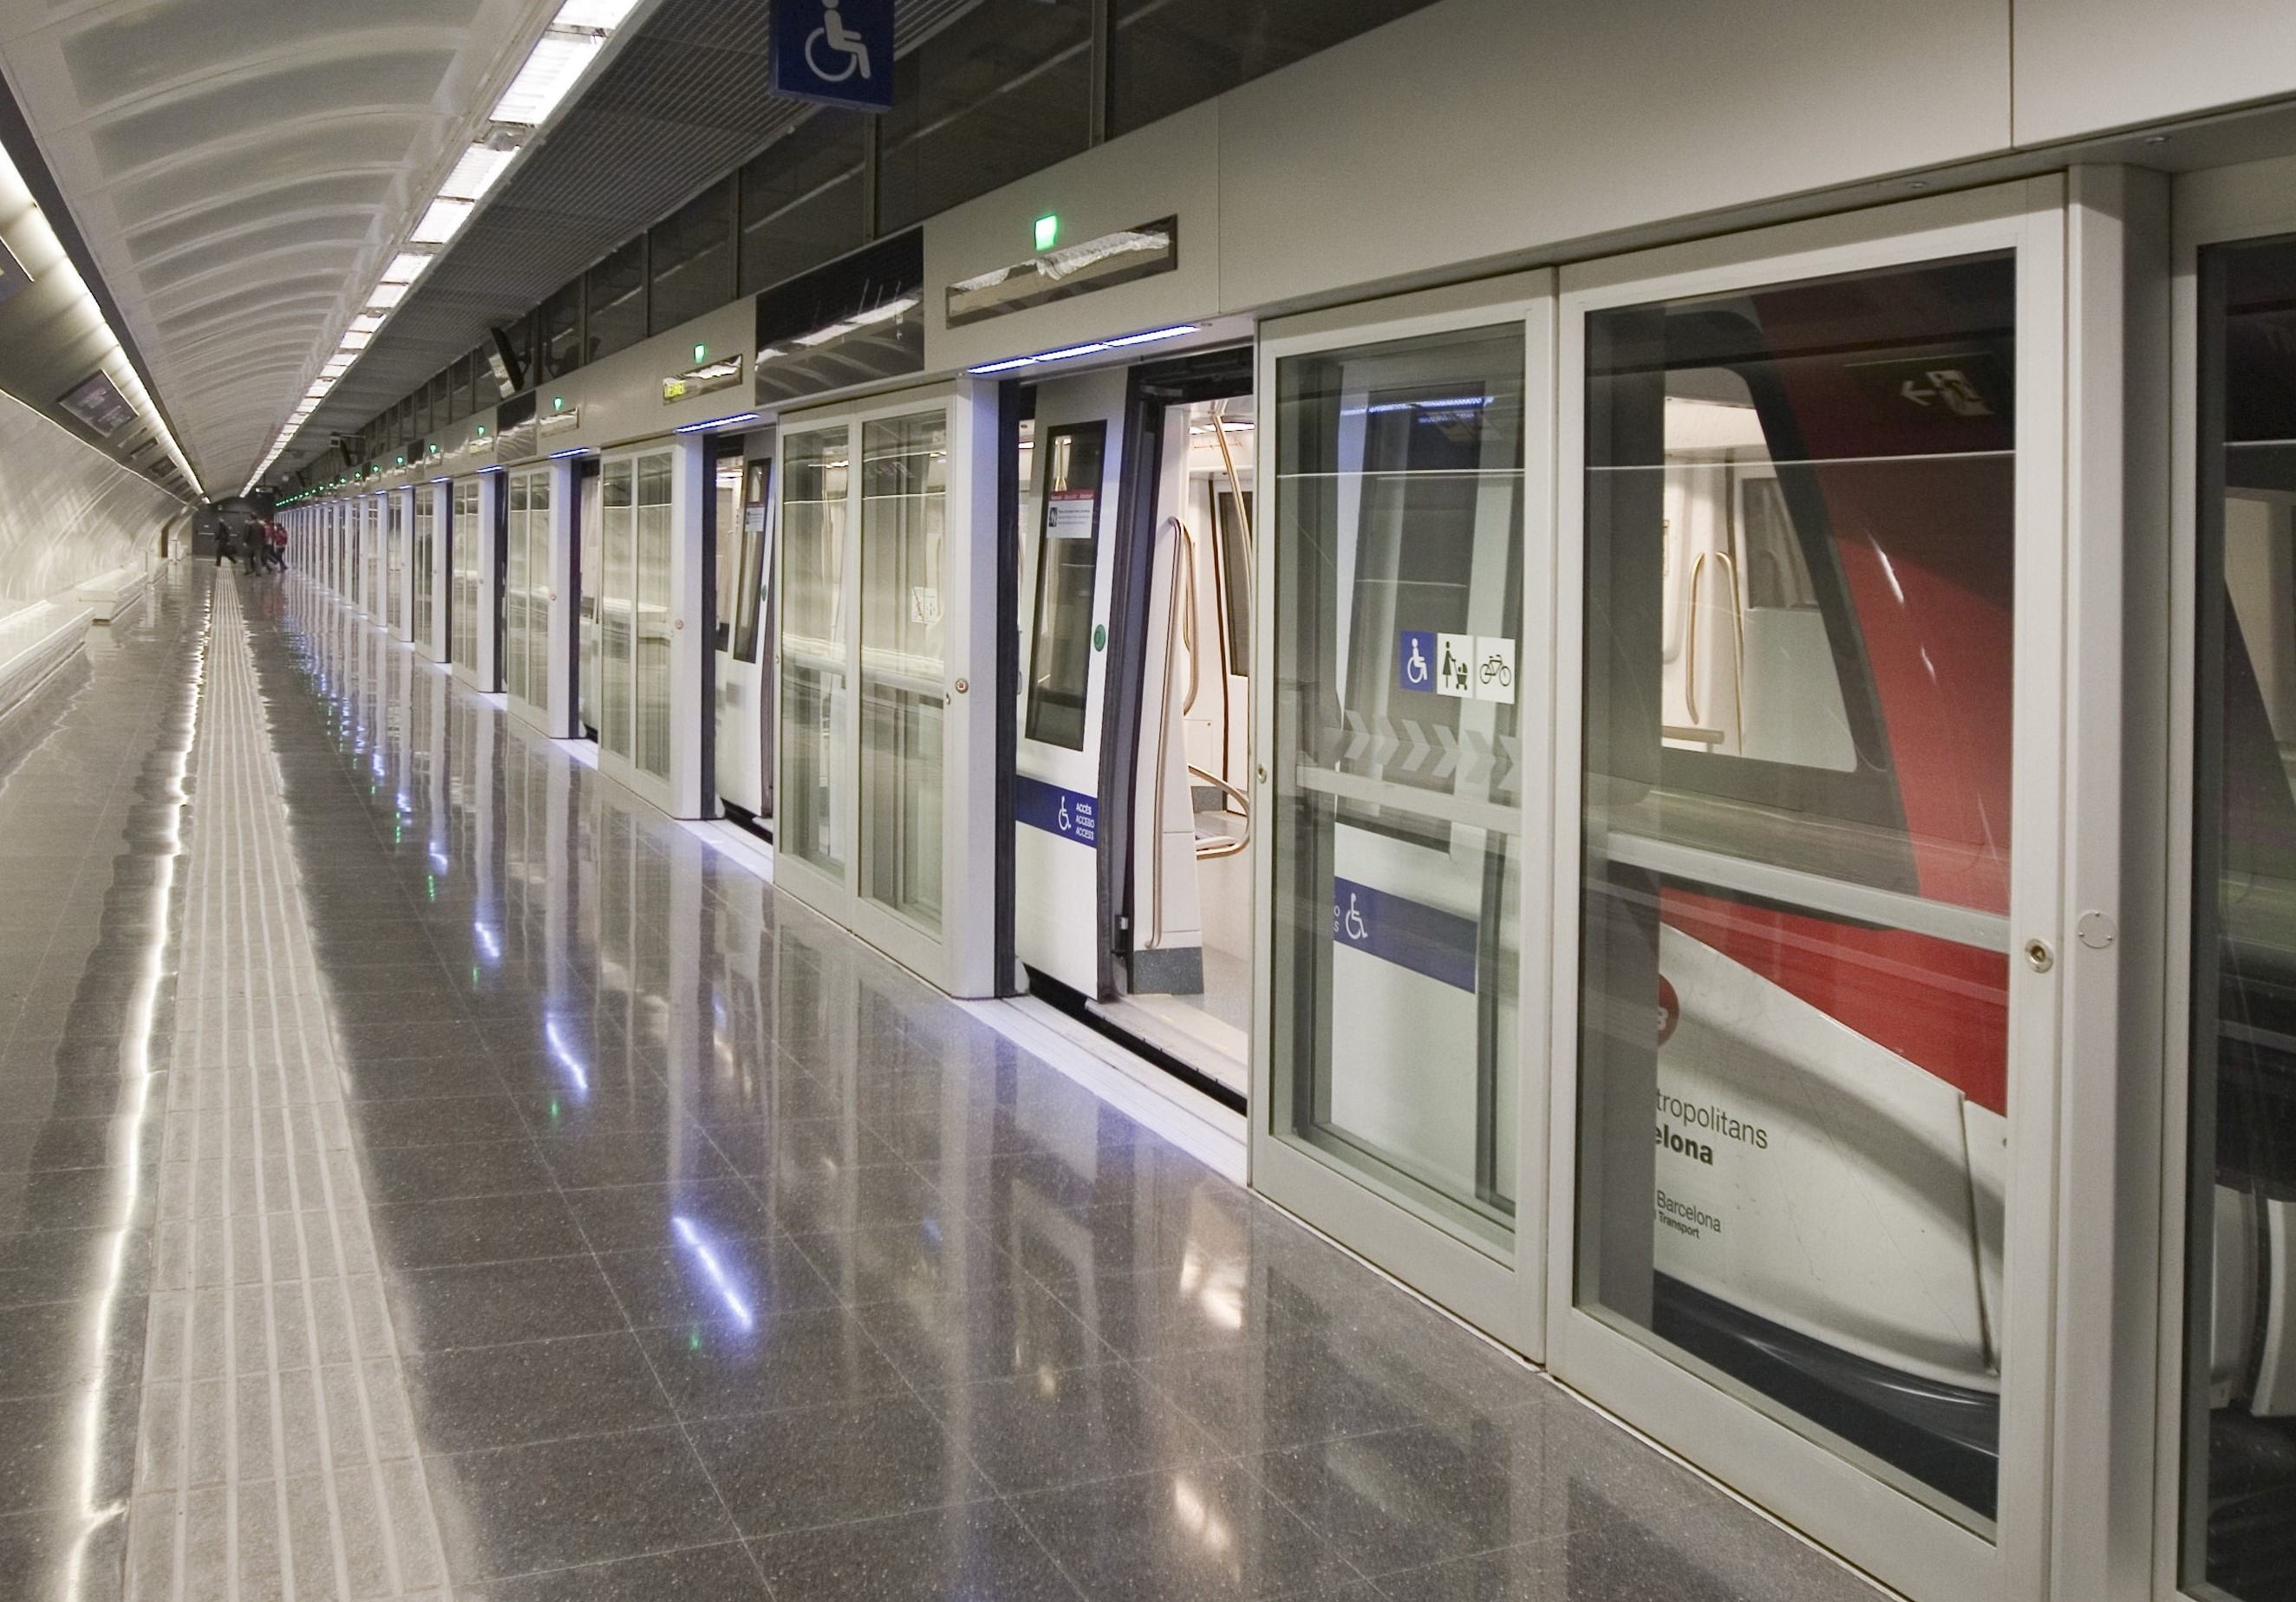
\includegraphics[keepaspectratio=true,width=\dimmin{}{\dimwidth{0.55}}]{images/Fig-1.a}{}%mdk
%mdk
\end{mdcenter}%mdk

%mdk-data-line={73}
\begin{mdcenter}%mdk

%mdk-data-line={74}
\noindent\mdline{74}\textbf{Figure 1.a.- Platform Screen Doors in Barcelona's subway (Line 9).}%mdk
%mdk
\end{mdcenter}%mdk

%mdk-data-line={77}
\noindent\mdline{77}The goal of PSD is to provide an automatic operation for the trains in a subway network. These trains operate 
autonomously, without a driver, and are coordinated with the PSD in such a way that, when they arrive at the 
platform of a station, both the PSD and the carriage doors open and close simultaneously.%mdk

%mdk-data-line={81}
\mdline{81}A typical module of PSD is composed by a pair of sliding door leaves, two adjacent panels, a threshold and a 
header box. Every sliding door consists of a glass panel (height of 2 – 2,2 m and 
width of 1 – 1,2 m), a metallic frame, a door guide and door hangers.%mdk

%mdk-data-line={85}
\mdline{85}Fire safety is becoming more and more relevant in the design of infrastructures. In the case of a subway station, 
a subway carriage constitutes the worst source of a fire, which may involve different parts of it and, therefore, 
the heat release rate (HRR, from now on) and its distribution in time may be very different, depending on the part that ignites.%mdk

%mdk-data-line={89}
\mdline{89}The Firestarr project is a European research program that took place in 1997, aimed at studying the fire development 
in rail and subway trains. This program stated that arson involving the interior of a train carriage was the main cause 
for a fire in European trains. As far as the UK is referred, in the period from 1992 to 2000, 2.911 fires occurred in trains, 
with a 77,8\% of the total involving passenger trains. Arson was responsible for the 56\% of these fires, which took place in 
urban areas in the 90\% of the cases.%mdk

%mdk-data-line={95}
\mdline{95}Some arson attacks in subway stations have caused multiple victims, as the case of the Daegu Subway (South Korea), which took 
place in 2003, causing the death of 192 civilians.%mdk

%mdk-data-line={98}
\mdline{98}The goal of the present study is to carry out an assessment of the effect on the evacuation conditions in a subway station, 
depending on the existence of PSD in an emergency situation because of a fire. Since arson has been documented as being the 
main cause of a fire in a subway carriage, the present study is focused on fires caused by such event.%mdk

%mdk-data-line={102}
\section{\mdline{102}2.\hspace*{0.5em}\mdline{102}Subway stations}\label{sec-subway-stations}%mdk%mdk

%mdk-data-line={104}
\noindent\mdline{104}In the present study, two types of stations have been considered:%mdk

%mdk-data-line={106}
\begin{itemize}[noitemsep,topsep=\mdcompacttopsep]%mdk

%mdk-data-line={106}
\item\mdline{106}\textbf{Cut and Cover stations.}\mdline{106}%mdk
%mdk
\end{itemize}%mdk

%mdk-data-line={108}
\noindent\mdline{108}Their main feature is the great volume inside them, which allows enough space to have both the escalators and the stairs 
in the platform, connecting to the mezzanine level, as shown in \mdline{109}\textbf{Figures 2.a-b}\mdline{109}.%mdk

%mdk-data-line={111}
\begin{mdcenter}%mdk

%mdk-data-line={112}
\noindent\mdline{112}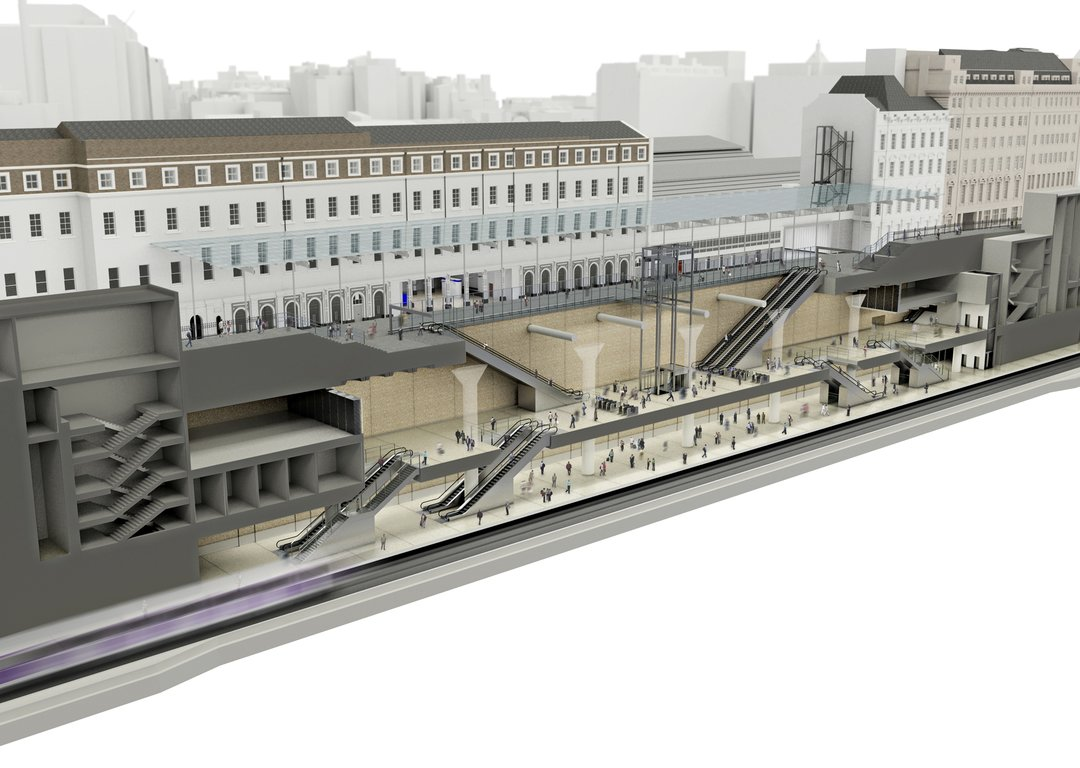
\includegraphics[keepaspectratio=true,width=\dimmin{}{\dimwidth{0.50}}]{images/Fig-2.a}{}%mdk
%mdk
\end{mdcenter}%mdk

%mdk-data-line={117}
\begin{mdcenter}%mdk

%mdk-data-line={118}
\noindent\mdline{118}\textbf{Figure 2.a.- Cut \& Cover station of Crossrail Paddington station in London (I).}%mdk
%mdk
\end{mdcenter}%mdk

%mdk-data-line={125}
\begin{mdcenter}%mdk

%mdk-data-line={126}
\noindent\mdline{126}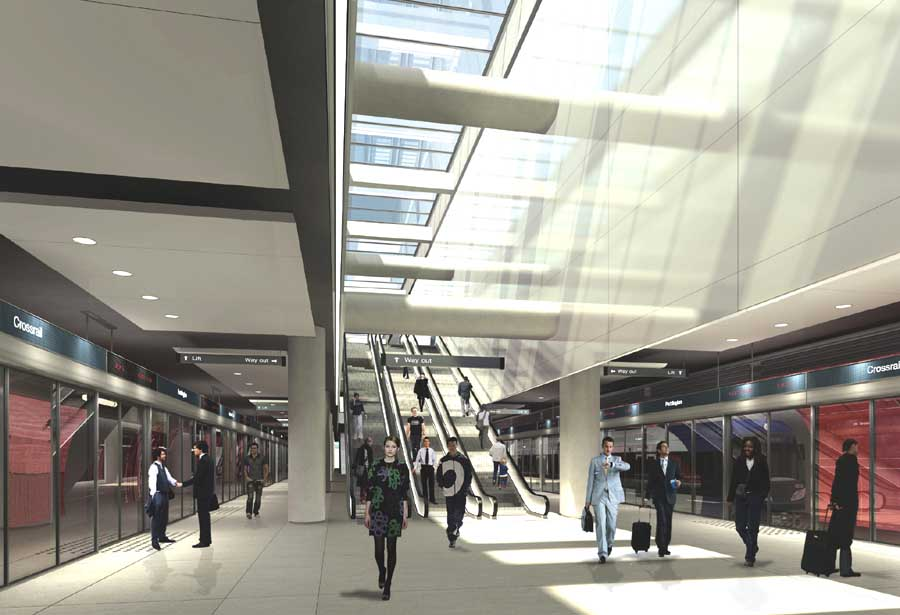
\includegraphics[keepaspectratio=true,width=\dimmin{}{\dimwidth{0.50}}]{images/Fig-2.b}{}%mdk
%mdk
\end{mdcenter}%mdk

%mdk-data-line={130}
\begin{mdcenter}%mdk

%mdk-data-line={131}
\noindent\mdline{131}\textbf{Figure 2.b.- Cut \& Cover station of Crossrail Paddington station in London (II)}\mdline{131}.%mdk
%mdk
\end{mdcenter}%mdk

%mdk-data-line={136}
\begin{itemize}[noitemsep,topsep=\mdcompacttopsep]%mdk

%mdk-data-line={136}
\item\mdline{136}\textbf{Cavern stations.}\mdline{136}%mdk
%mdk
\end{itemize}%mdk

%mdk-data-line={138}
\noindent\mdline{138}Their main feature is the lack of space inside them, which usually forces both 
the escalators and stairs to be placed in other places, being connected to the 
platforms through passageways, as shown in \mdline{140}\textbf{Figures 2.c-d}\mdline{140}.%mdk

%mdk-data-line={142}
\begin{mdcenter}%mdk

%mdk-data-line={143}
\noindent\mdline{143}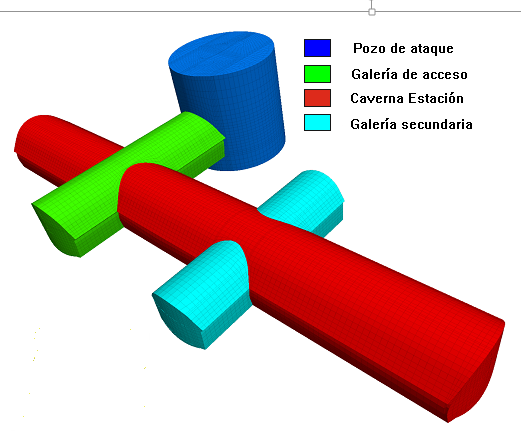
\includegraphics[keepaspectratio=true,width=\dimmin{}{\dimwidth{0.40}}]{images/Fig-2.c}{}%mdk
%mdk
\end{mdcenter}%mdk

%mdk-data-line={147}
\begin{mdcenter}%mdk

%mdk-data-line={148}
\noindent\mdline{148}\textbf{Figure 2.c.- Design of subway station of Line 6 (Santiago, Chile) done by Geocontrol.}%mdk
%mdk
\end{mdcenter}%mdk

%mdk-data-line={151}
\begin{mdcenter}%mdk

%mdk-data-line={152}
\noindent\mdline{152}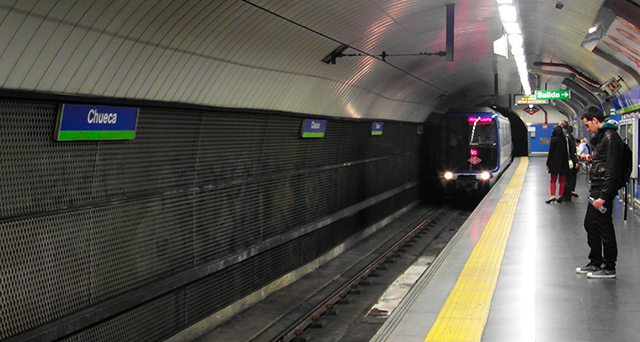
\includegraphics[keepaspectratio=true,width=\dimmin{}{\dimwidth{0.40}}]{images/Fig-2.d}{}\mdline{152}%mdk
%mdk
\end{mdcenter}%mdk

%mdk-data-line={157}
\begin{mdcenter}%mdk

%mdk-data-line={158}
\noindent\mdline{158}\textbf{Figure 2.d.- Platform in Line 5 Chueca station (Madrid, Spain).}%mdk
%mdk
\end{mdcenter}%mdk

%mdk-data-line={161}
\noindent\mdline{161}The comparison of both types of stations lets one foresee that the behavior of the 
smoke will probably be different in each station.%mdk

%mdk-data-line={164}
\section{\mdline{164}3.\hspace*{0.5em}\mdline{164}Modeling of the fire event}\label{sec-modeling-of-the-fire-event}%mdk%mdk

%mdk-data-line={166}
\noindent\mdline{166}In order to design correctly the fire safety requirements of a station, it is vital 
to have an accurate fire event modelling. According to the European Standard EN 45545 
and to the ASHRAE Handbook, a fire from a new, hardened vehicle of a train can have 
an HRR of around 10 MW. The tests of fire behavior done in the Eureka project 
framework allow to have the HRR of a subway carriage, as shown in \mdline{170}\textbf{Figure 3.a}\mdline{170}.%mdk

%mdk-data-line={172}
\begin{mdcenter}%mdk

%mdk-data-line={173}
\noindent\mdline{173}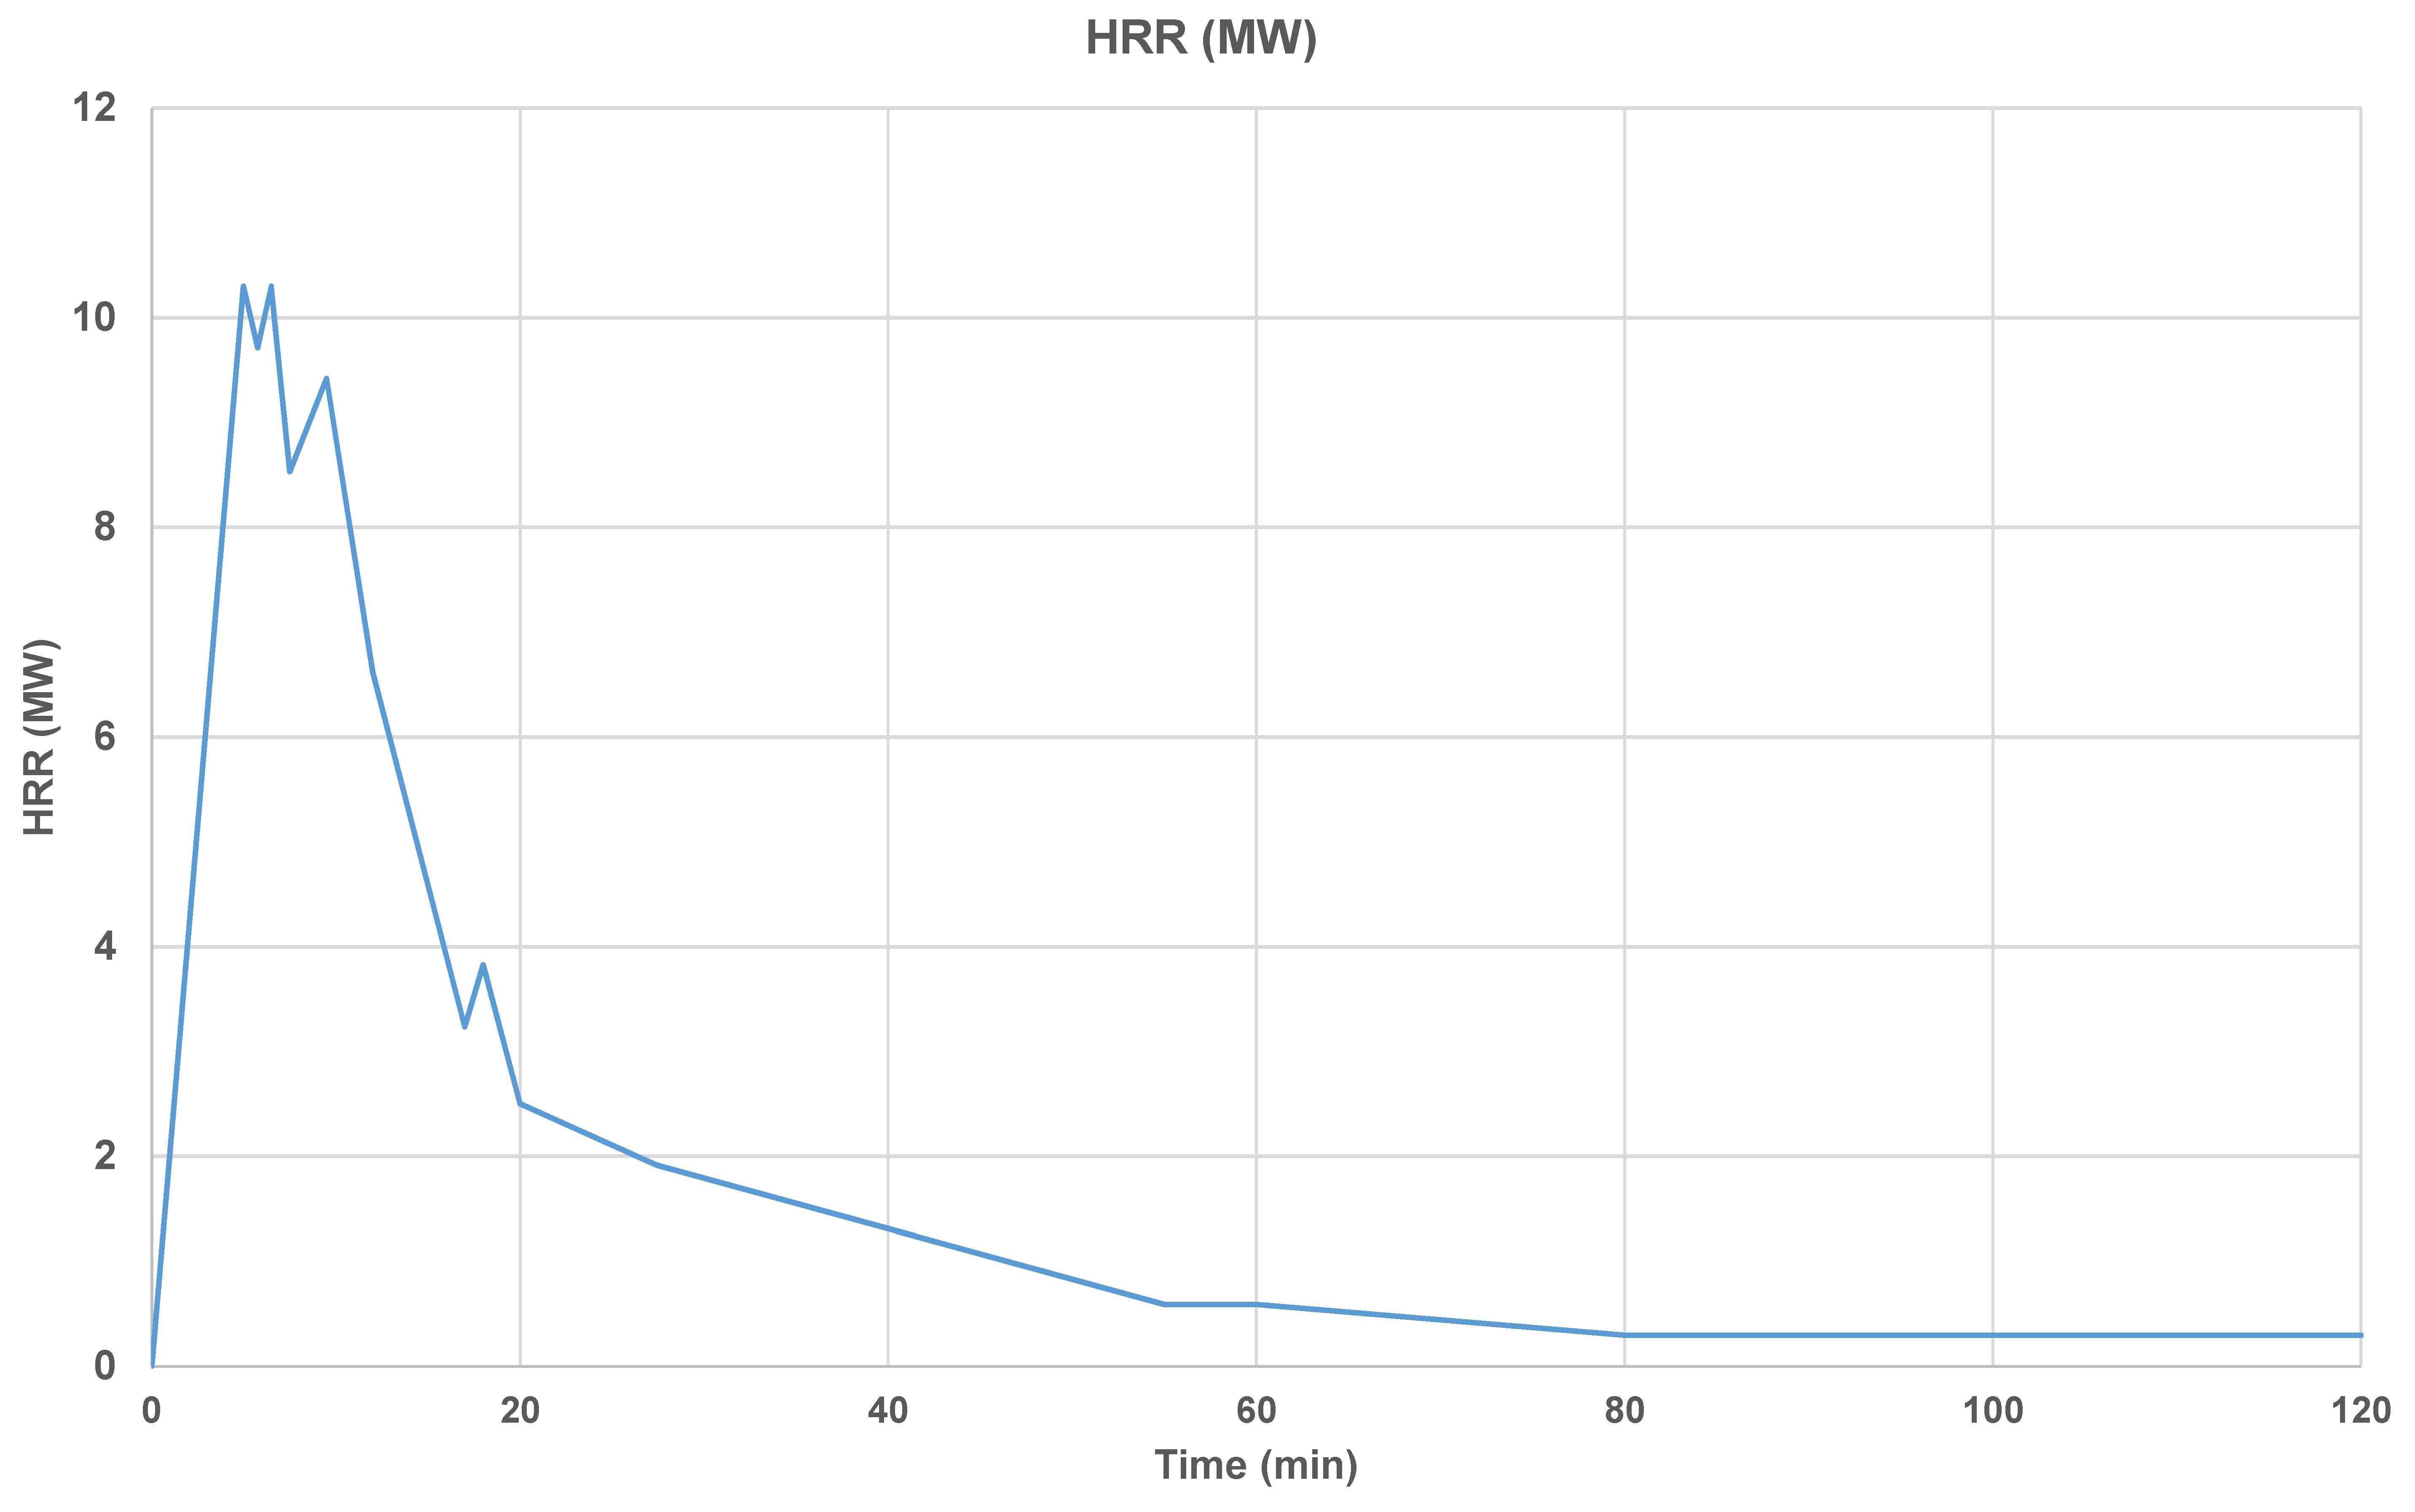
\includegraphics[keepaspectratio=true,width=\dimmin{}{\dimwidth{0.45}}]{images/Fig-3.a}{}%mdk
%mdk
\end{mdcenter}%mdk

%mdk-data-line={177}
\begin{mdcenter}%mdk

%mdk-data-line={178}
\noindent\mdline{178}\textbf{Figure 3.a.- HRR of a subway carriage.}%mdk
%mdk
\end{mdcenter}%mdk

%mdk-data-line={181}
\noindent\mdline{181}The HRR curve shown in Figure 3.a refers to a fire due to an arson attack 
inside a subway carriage.%mdk

%mdk-data-line={184}
\mdline{184}The next step consists in creating a geometrical model that reproduces 
the shape, volume and features of both types of stations, which has been 
carried out with Pyrosim, as shown in \mdline{186}\textbf{Figures 3.b-c}\mdline{186}.%mdk

%mdk-data-line={188}
\begin{mdcenter}%mdk

%mdk-data-line={189}
\noindent\mdline{189}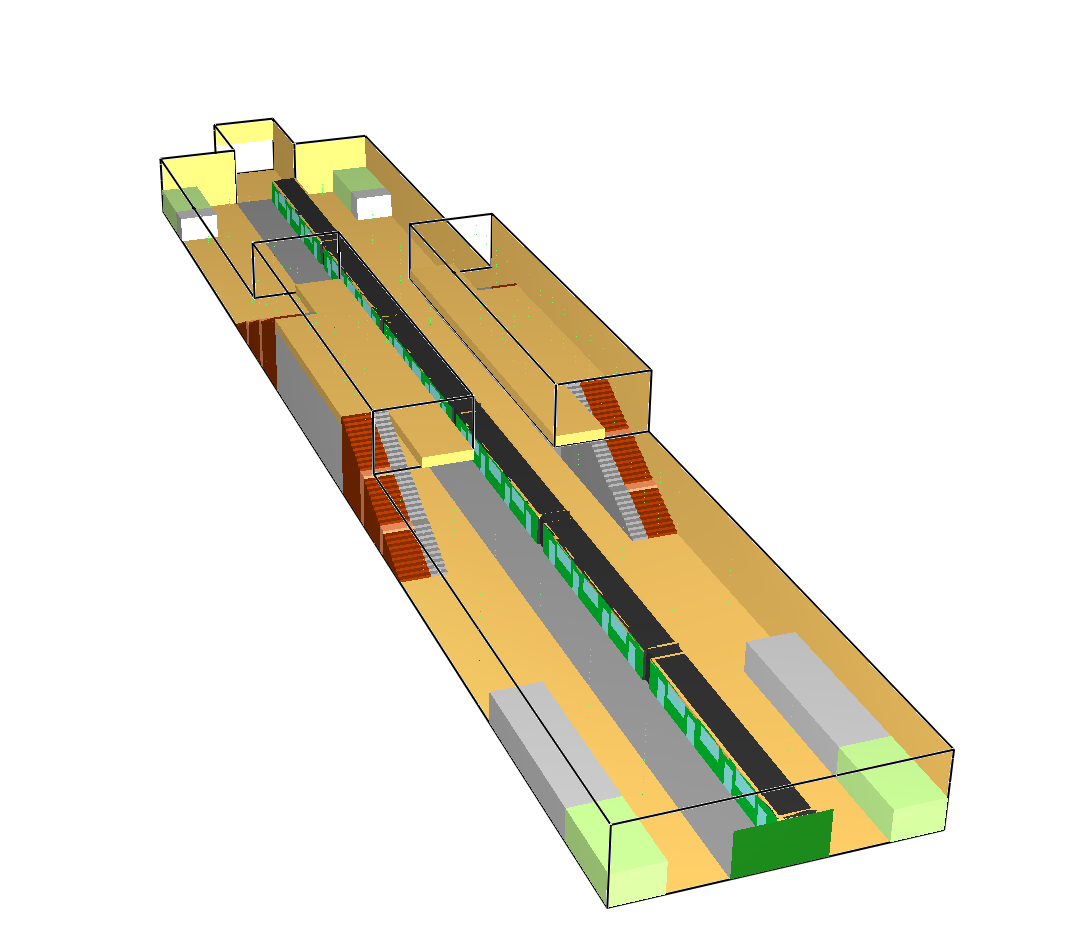
\includegraphics[keepaspectratio=true,width=\dimmin{}{\dimwidth{0.45}}]{images/Fig-3.b}{}%mdk
%mdk
\end{mdcenter}%mdk

%mdk-data-line={193}
\begin{mdcenter}%mdk

%mdk-data-line={194}
\noindent\mdline{194}\textbf{Figure 3.b.- Geometrical model for Cut \& Cover station.}%mdk
%mdk
\end{mdcenter}%mdk

%mdk-data-line={197}
\begin{mdcenter}%mdk

%mdk-data-line={198}
\noindent\mdline{198}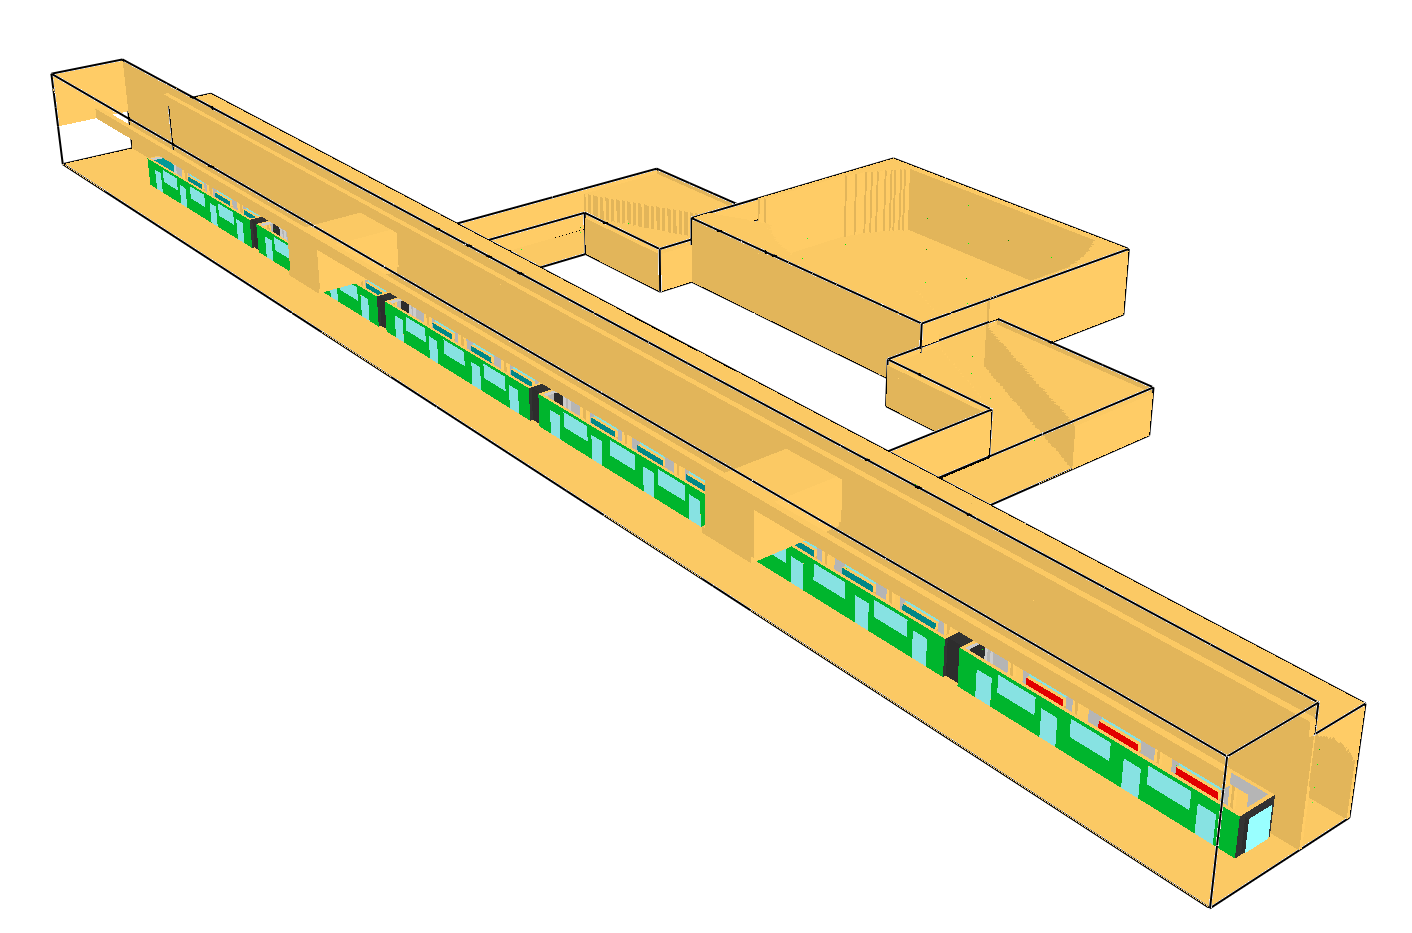
\includegraphics[keepaspectratio=true,width=\dimmin{}{\dimwidth{0.45}}]{images/Fig-3.c}{}%mdk
%mdk
\end{mdcenter}%mdk

%mdk-data-line={202}
\begin{mdcenter}%mdk

%mdk-data-line={203}
\noindent\mdline{203}\textbf{Figure 3.c.- Geometrical model for Cavern station.}%mdk
%mdk
\end{mdcenter}%mdk

%mdk-data-line={210}
\noindent\mdline{210}Once the geometry has been created, the ventilation strategy is the last step 
to define the operation of a station in a fire event. An assessment will be 
carried out between two ventilation strategies in a Cut \mdline{212}\&\mdline{212} Cover station and in a 
Cavern station in case of a fire event due to an arson attack in the inside of a 
carriage.%mdk

%mdk-data-line={216}
\begin{itemize}[noitemsep,topsep=\mdcompacttopsep]%mdk

%mdk-data-line={216}
\item\mdline{216}\textbf{Strategy S.T. A.}\mdline{216}%mdk
%mdk
\end{itemize}%mdk

%mdk-data-line={218}
\noindent\mdline{218}There are PSD in the platform, isolating the platform from the trackway when 
there is no train in the station. In this case, a train has just arrived to 
the station and the fire has just begun to take place inside the last carriage.%mdk

%mdk-data-line={222}
\mdline{222}The train doors are open and so the PSD, which allows most of the smoke from the 
carriage to invade the platform, where there is an amount of passengers. The rest 
of the smoke is isolated in the volume of the tracks, because of the PSD, which 
constitute a physical barrier.%mdk

%mdk-data-line={227}
\mdline{227}After 30s, the fire in the station is detected, two different ventilation systems 
get activated: the station and the tunnel ventilation system. Thus, the smoke in the 
platform is exhausted by the station ventilation system, while fire in the tracks 
region is exhausted by the tunnel ventilation system.%mdk

%mdk-data-line={232}
\mdline{232}The station ventilation system connects with the platform through a ventilation duct 
placed in the high part of the platform, as it is shown in the \mdline{233}\textbf{Figure 3.d}\mdline{233}.%mdk

%mdk-data-line={235}
\begin{mdcenter}%mdk

%mdk-data-line={236}
\noindent\mdline{236}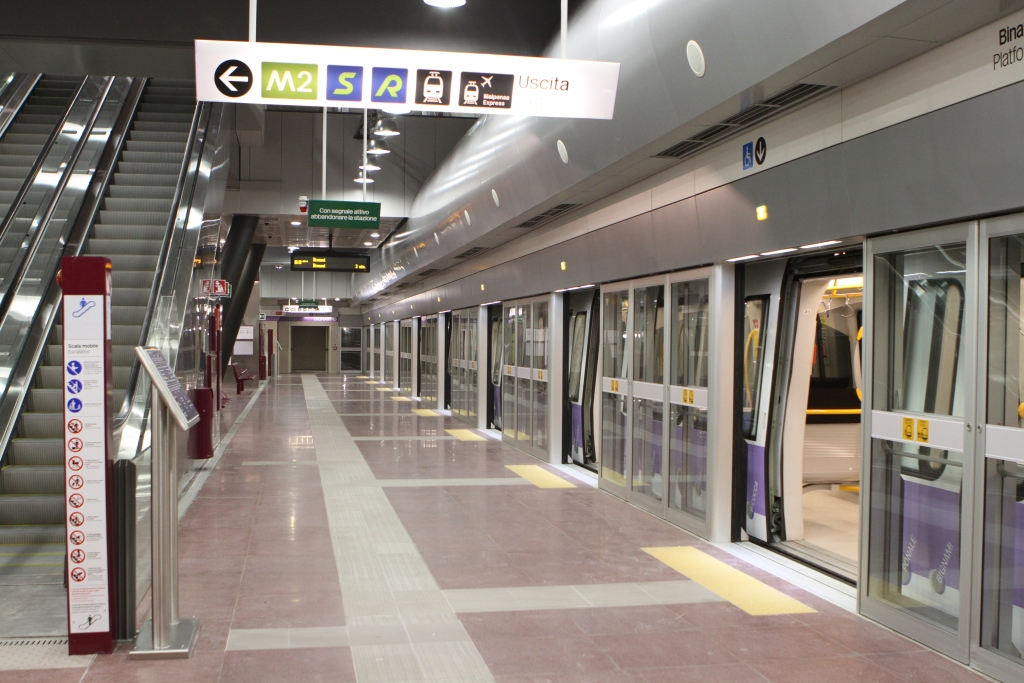
\includegraphics[keepaspectratio=true,width=\dimmin{}{\dimwidth{0.50}}]{images/Fig-3.d}{}%mdk
%mdk
\end{mdcenter}%mdk

%mdk-data-line={240}
\begin{mdcenter}%mdk

%mdk-data-line={241}
\noindent\mdline{241}\textbf{Figure 3.d. – Exhaust grids in the M5 subway line in Milan (Italy).}%mdk
%mdk
\end{mdcenter}%mdk

%mdk-data-line={244}
\noindent\mdline{244}The exhaust rates have been calculated with the formulas included in the NFPA 92 
and are the following ones:%mdk

%mdk-data-line={247}
\begin{mdcenter}%mdk

%mdk-data-line={248}
\noindent\mdline{248}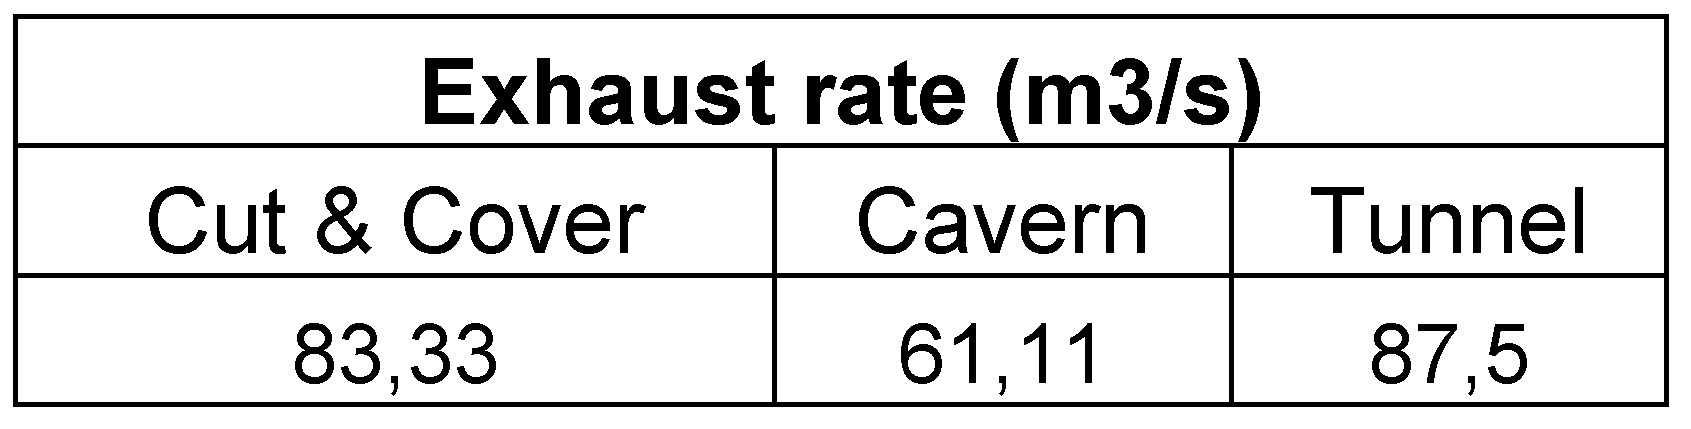
\includegraphics[keepaspectratio=true,width=\dimmin{}{\dimwidth{0.35}}]{images/Table-3.I}{}%mdk
%mdk
\end{mdcenter}%mdk

%mdk-data-line={252}
\begin{mdcenter}%mdk

%mdk-data-line={253}
\noindent\mdline{253}\textbf{Table 3.I.- Exhaust rates in the cases with PSD in the stations.}%mdk
%mdk
\end{mdcenter}%mdk

%mdk-data-line={256}
\begin{itemize}[noitemsep,topsep=\mdcompacttopsep]%mdk

%mdk-data-line={256}
\item\mdline{256}\textbf{Strategy S.T. B.}\mdline{256}%mdk
%mdk
\end{itemize}%mdk

%mdk-data-line={258}
\noindent\mdline{258}In this case, there are no PSD in any of the stations.%mdk

%mdk-data-line={260}
\mdline{260}The schedule of the events is the same: a train arrives and an arson attack is 
carried out in the last carriage. In this case, due to the absence of PSD, the 
smoke invades both platforms almost simultaneously, as no physical barrier protects 
the passengers in the station.%mdk

%mdk-data-line={265}
\mdline{265}The ventilation strategy is based on exhausting the whole smoke generation with the 
tunnel ventilation system. A station exhaust is ruled out in this case, as it would 
interfere with the tunnel exhaust, jeopardizing the operation of each other, something 
that didn’t happen with strategy S.T. A, since PSD are considered in the station. 
Thus, the exhaust rate considered is the following one:%mdk

%mdk-data-line={271}
\begin{mdcenter}%mdk

%mdk-data-line={272}
\noindent\mdline{272}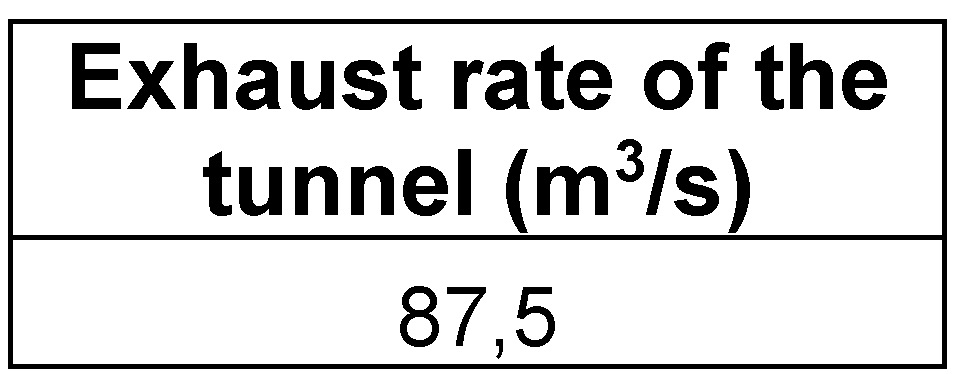
\includegraphics[keepaspectratio=true,width=\dimmin{}{\dimwidth{0.22}}]{images/Table-3.II}{}%mdk
%mdk
\end{mdcenter}%mdk

%mdk-data-line={276}
\begin{mdcenter}%mdk

%mdk-data-line={277}
\noindent\mdline{277}\textbf{Table 3.II. – Exhaust rates in the cases without PSD in the stations.}%mdk
%mdk
\end{mdcenter}%mdk

%mdk-data-line={280}
\section{\mdline{280}4.\hspace*{0.5em}\mdline{280}Assessment}\label{sec-assessment}%mdk%mdk

%mdk-data-line={282}
\noindent\mdline{282}The comparison of both strategies will be carried out according to the NFPA 130 
standard, which considers the temperature, the CO concentration and the visibility 
as the main factors involved in the evacuation process, stating conditions for the 
health of the passengers, as shown in \mdline{285}\textbf{Tables 4.I}\mdline{285} and \mdline{285}\textbf{4.II}\mdline{285}.%mdk

%mdk-data-line={287}
\begin{mdcenter}%mdk

%mdk-data-line={288}
\noindent\mdline{288}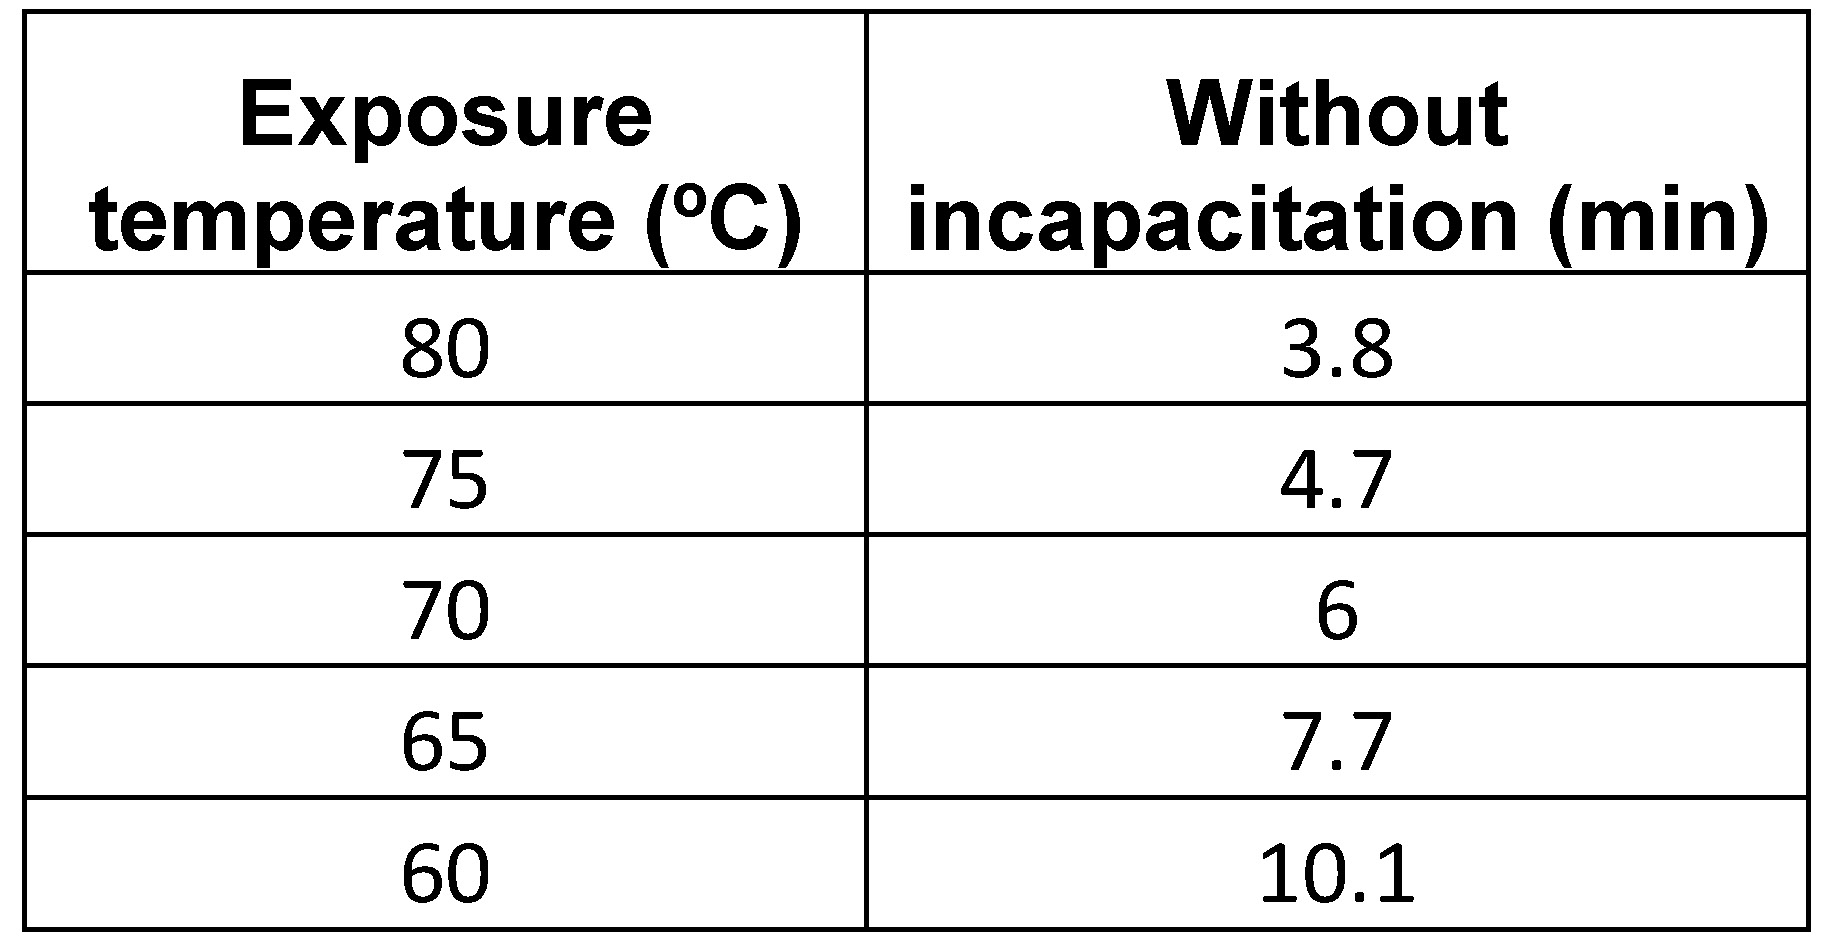
\includegraphics[keepaspectratio=true,width=\dimmin{}{\dimwidth{0.40}}]{images/Table-4.I}{}%mdk
%mdk
\end{mdcenter}%mdk

%mdk-data-line={292}
\begin{mdcenter}%mdk

%mdk-data-line={293}
\noindent\mdline{293}\textbf{Table 4.I. – Maximum exposure time to high levels of temperature.}%mdk
%mdk
\end{mdcenter}%mdk

%mdk-data-line={296}
\begin{mdcenter}%mdk

%mdk-data-line={297}
\noindent\mdline{297}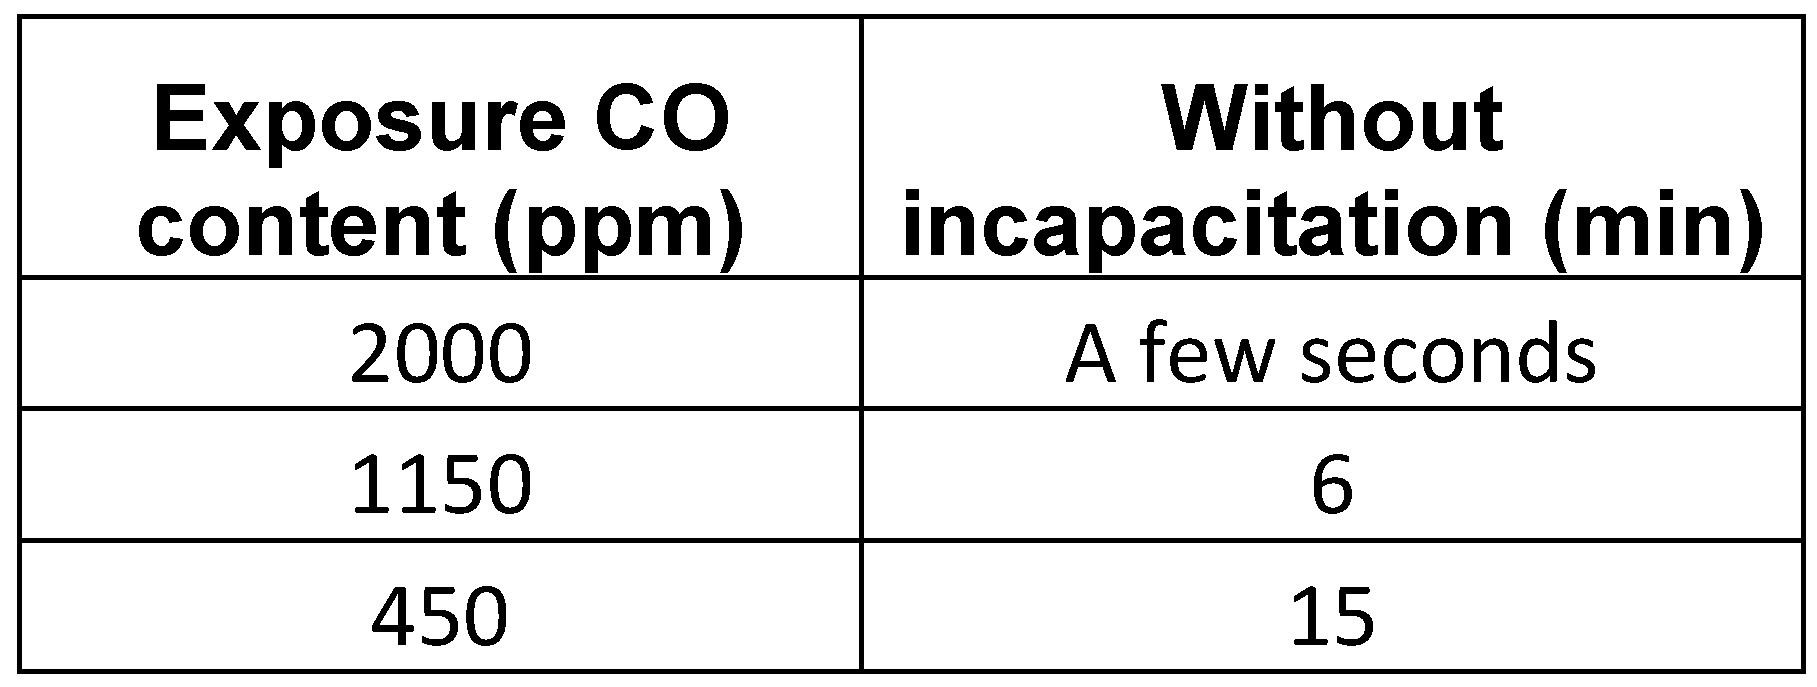
\includegraphics[keepaspectratio=true,width=\dimmin{}{\dimwidth{0.40}}]{images/Table-4.II}{}%mdk
%mdk
\end{mdcenter}%mdk

%mdk-data-line={301}
\begin{mdcenter}%mdk

%mdk-data-line={302}
\noindent\mdline{302}\textbf{Table 4.II. – Maximum exposure time to high levels of CO concentration.}%mdk
%mdk
\end{mdcenter}%mdk

%mdk-data-line={305}
\noindent\mdline{305}The visibility affects the evacuation process, since a reduced level of this variable 
means that the passengers move slower than if there were no smoke. It is required for 
doors and walls to be discernible at a distance of 10m.%mdk

%mdk-data-line={309}
\mdline{309}Apart from the visibility, the required time for the complete evacuation of the station 
will be assessed, surveilling if any passenger faces lethal conditions with an 
exposition that surpasses the values outlined in Tables 4.I and 4.II.%mdk

%mdk-data-line={313}
\subsection{\mdline{313}4.1.\hspace*{0.5em}\mdline{313}Simulations in the Cut \mdline{313}\&\mdline{313} Cover station.}\label{sec-simulations-in-the-cut-cover-station}%mdk%mdk

%mdk-data-line={315}
\noindent\mdline{315}Some devices for the control of temperature, CO concentration and visibility have been 
placed all along each platform, so that their value can be known in the egress routes 
and inside the carriages during the fire.%mdk

%mdk-data-line={319}
\begin{itemize}[noitemsep,topsep=\mdcompacttopsep]%mdk

%mdk-data-line={319}
\item\mdline{319}\textbf{Main differences between both strategies.}\mdline{319}%mdk
%mdk
\end{itemize}%mdk

%mdk-data-line={321}
\noindent\mdline{321}The fire takes place in the inside of the last carriage on the right, as shown 
in \mdline{322}\textbf{Figure 4.1.a}\mdline{322}.%mdk

%mdk-data-line={324}
\begin{mdcenter}%mdk

%mdk-data-line={325}
\noindent\mdline{325}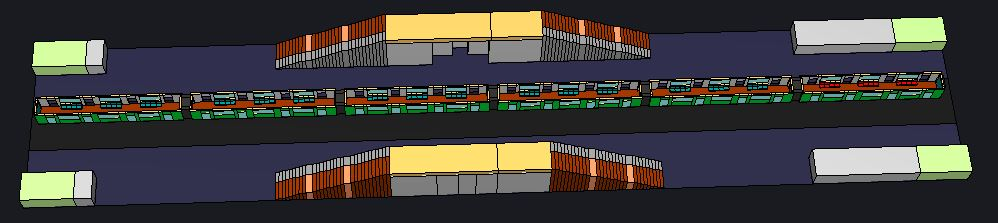
\includegraphics[keepaspectratio=true,width=\dimmin{}{\dimwidth{0.80}}]{images/Fig-4.1.a}{}%mdk
%mdk
\end{mdcenter}%mdk

%mdk-data-line={329}
\begin{mdcenter}%mdk

%mdk-data-line={330}
\noindent\mdline{330}\textbf{Figure 4.1.a. – Cut \& Cover fire model created with Pyrosim.}%mdk
%mdk
\end{mdcenter}%mdk

%mdk-data-line={333}
\noindent\mdline{333}In the case of strategy S.T. A, the passengers on the platform PL. B are completely 
isolated from the fire and the smoke. However, the passengers on Platform PL. A 
(the one close to the train) must face the smoke coming from the inside of the 
carriage.%mdk

%mdk-data-line={338}
\mdline{338}In the case of strategy B, both the passengers in platforms PL. A and PL. B are exposed 
to the fire and must face harsh conditions during the evacuation, in contrast with 
the situation described with the strategy S.T. A.%mdk

%mdk-data-line={342}
\begin{itemize}[noitemsep,topsep=\mdcompacttopsep]%mdk

%mdk-data-line={342}
\item\mdline{342}\textbf{Means of egress}\mdline{342}.%mdk
%mdk
\end{itemize}%mdk

%mdk-data-line={344}
\noindent\mdline{344}The passengers on each platform have four escape routes (E.R., from now on), as shown 
in \mdline{345}\textbf{Figure 4.1.a}\mdline{345}.%mdk

%mdk-data-line={347}
\begin{itemize}[noitemsep,topsep=\mdcompacttopsep]%mdk

%mdk-data-line={347}
\item\mdline{347}E.R. 1: toward the emergency door on the right side.%mdk

%mdk-data-line={348}
\item\mdline{348}E.R. 2: toward the escalators and stairs on the right side.%mdk

%mdk-data-line={349}
\item\mdline{349}E.R. 3: toward the escalators and stairs on the left side.%mdk

%mdk-data-line={350}
\item\mdline{350}E.R. 4: toward the emergency door on the left side of platform.%mdk
%mdk
\end{itemize}%mdk

%mdk-data-line={352}
\noindent\mdline{352}The region in front of the vandalized carriage is the one most affected by the fire.%mdk

%mdk-data-line={354}
\begin{itemize}[noitemsep,topsep=\mdcompacttopsep]%mdk

%mdk-data-line={354}
\item\mdline{354}\textbf{Development of the fire}\mdline{354}.%mdk
%mdk
\end{itemize}%mdk

%mdk-data-line={356}
\noindent\mdline{356}All the 6 carriages are connected to each other, what facilitates the smoke to invade 
the whole train, affecting all the people inside of it.%mdk

%mdk-data-line={359}
\mdline{359}Every carriage is built with 6 windows (3 per side), which break out when the temperature 
reaches 470ºC. This affects the development of the fire event, since the smoke finds a 
new way to escape from the train, heading to an isolated volume, not affecting the passengers.%mdk

%mdk-data-line={363}
\mdline{363}The variables that affect the evacuation of passengers are the temperature, concentration of CO 
and visibility.  In both strategies it has been verified that smoke tend to move to the 
upper level of the platforms because of the buoyancy effect. Thus, lethal levels of 
temperature and CO concentration are only reached inside the vandalized carriage, as 
shown in \mdline{367}\textbf{Figure 4.1.b}\mdline{367}, or in the highest part of the platform, far from a passenger, 
as shown in \mdline{368}\textbf{Figure 4.1.c}\mdline{368}.%mdk

%mdk-data-line={371}
\begin{mdcenter}%mdk

%mdk-data-line={372}
\noindent\mdline{372}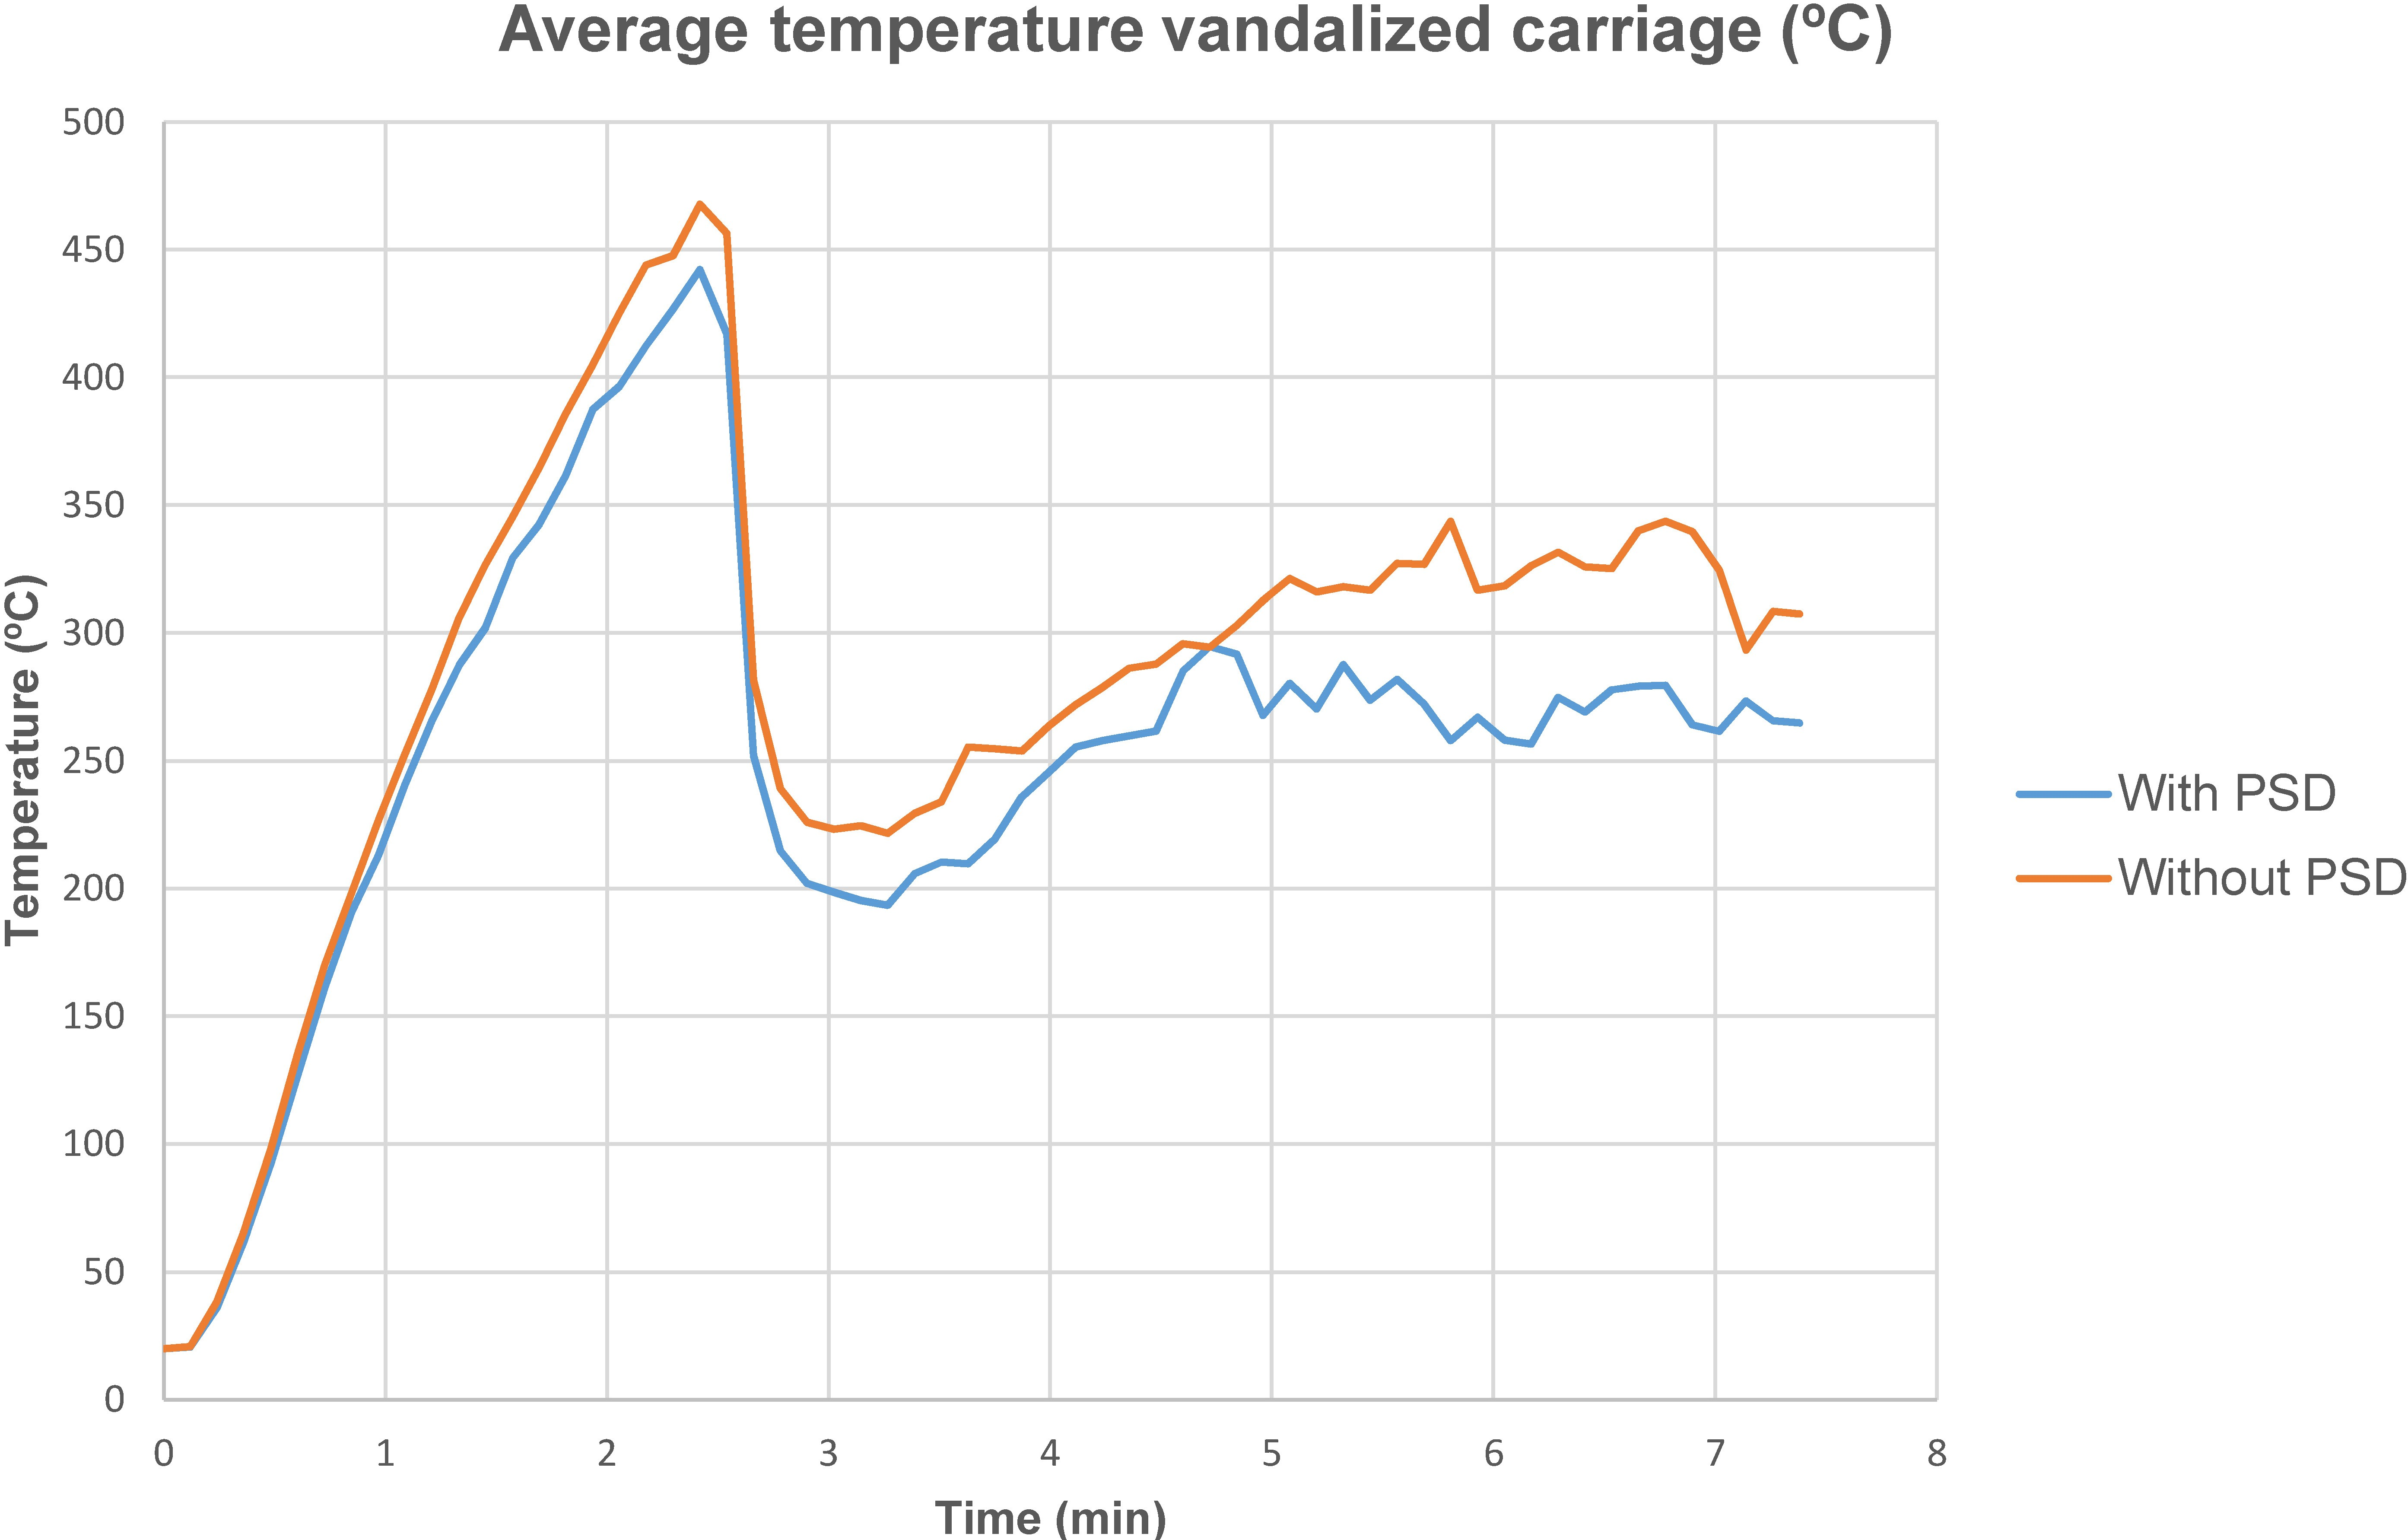
\includegraphics[keepaspectratio=true,width=\dimmin{}{\dimwidth{0.55}}]{images/Fig-4.1.b}{}%mdk
%mdk
\end{mdcenter}%mdk

%mdk-data-line={375}
\begin{mdcenter}%mdk

%mdk-data-line={376}
\noindent\mdline{376}\textbf{Figure 4.1.b. – Average temperature in the vandalized carriage at a height of 2m.}%mdk
%mdk
\end{mdcenter}%mdk

%mdk-data-line={381}
\noindent\mdline{381}The reason for the rapid decrease of the temperature in the inside of the carriage 
is that the threshold temperature is reached close to the windows, which break out, 
allowing the smoke to leave the carriage through these places.%mdk

%mdk-data-line={385}
\begin{mdcenter}%mdk

%mdk-data-line={386}
\noindent\mdline{386}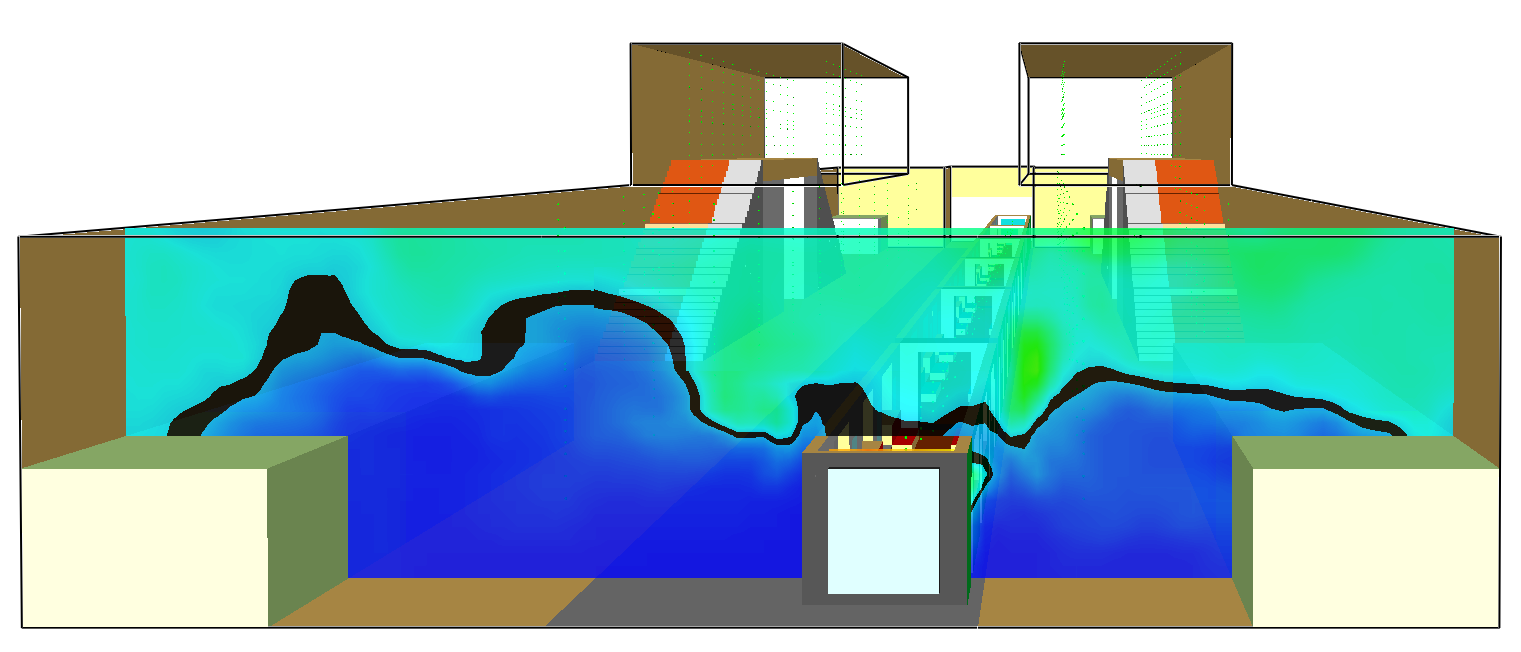
\includegraphics[keepaspectratio=true,width=\dimmin{}{\dimwidth{0.55}}]{images/Fig-4.1.c}{}%mdk
%mdk
\end{mdcenter}%mdk

%mdk-data-line={390}
\begin{mdcenter}%mdk

%mdk-data-line={391}
\noindent\mdline{391}\textbf{Figure 4.1.c. – Temperature in Cut \& Cover stations without PSD 
(t=6min, 80ºC in bold).}%mdk
%mdk
\end{mdcenter}%mdk

%mdk-data-line={395}
\noindent\mdline{395}The highest levels of temperature in the platform without PSD are of 150ºC, 
but at a height far from any passenger, as \mdline{396}\textbf{Figure 4.1.c}\mdline{396} shows.%mdk

%mdk-data-line={398}
\mdline{398}The highest temperatures that passengers must face without PSD are of 80ºC 
in the stairs on the right side of the platform, but during less time than 
3,8 min, which is the threshold time to be considered lethal. In contrast, 
with PSD, the maximum temperature is 80ºC, but only in places close to the 
vandalized carriage.%mdk

%mdk-data-line={404}
\mdline{404}The station’s ventilation has a positive effect on safety, because the air 
exhausted is replaced by air through the connection between the stairs and 
the mezzanine level, enhancing the evacuating conditions in the stairs, 
since the passengers’ egress direction is opposite to the air direction.%mdk

%mdk-data-line={409}
\mdline{409}The effect of the smoke on the visibility is more notorious, and great 
differences are appreciated between both strategies, as presented in 
\mdline{411}\textbf{Figure 4.1.d}\mdline{411} in front of the vandalized carriage, where the conditions 
are harsher.%mdk

%mdk-data-line={414}
\begin{mdcenter}%mdk

%mdk-data-line={415}
\noindent\mdline{415}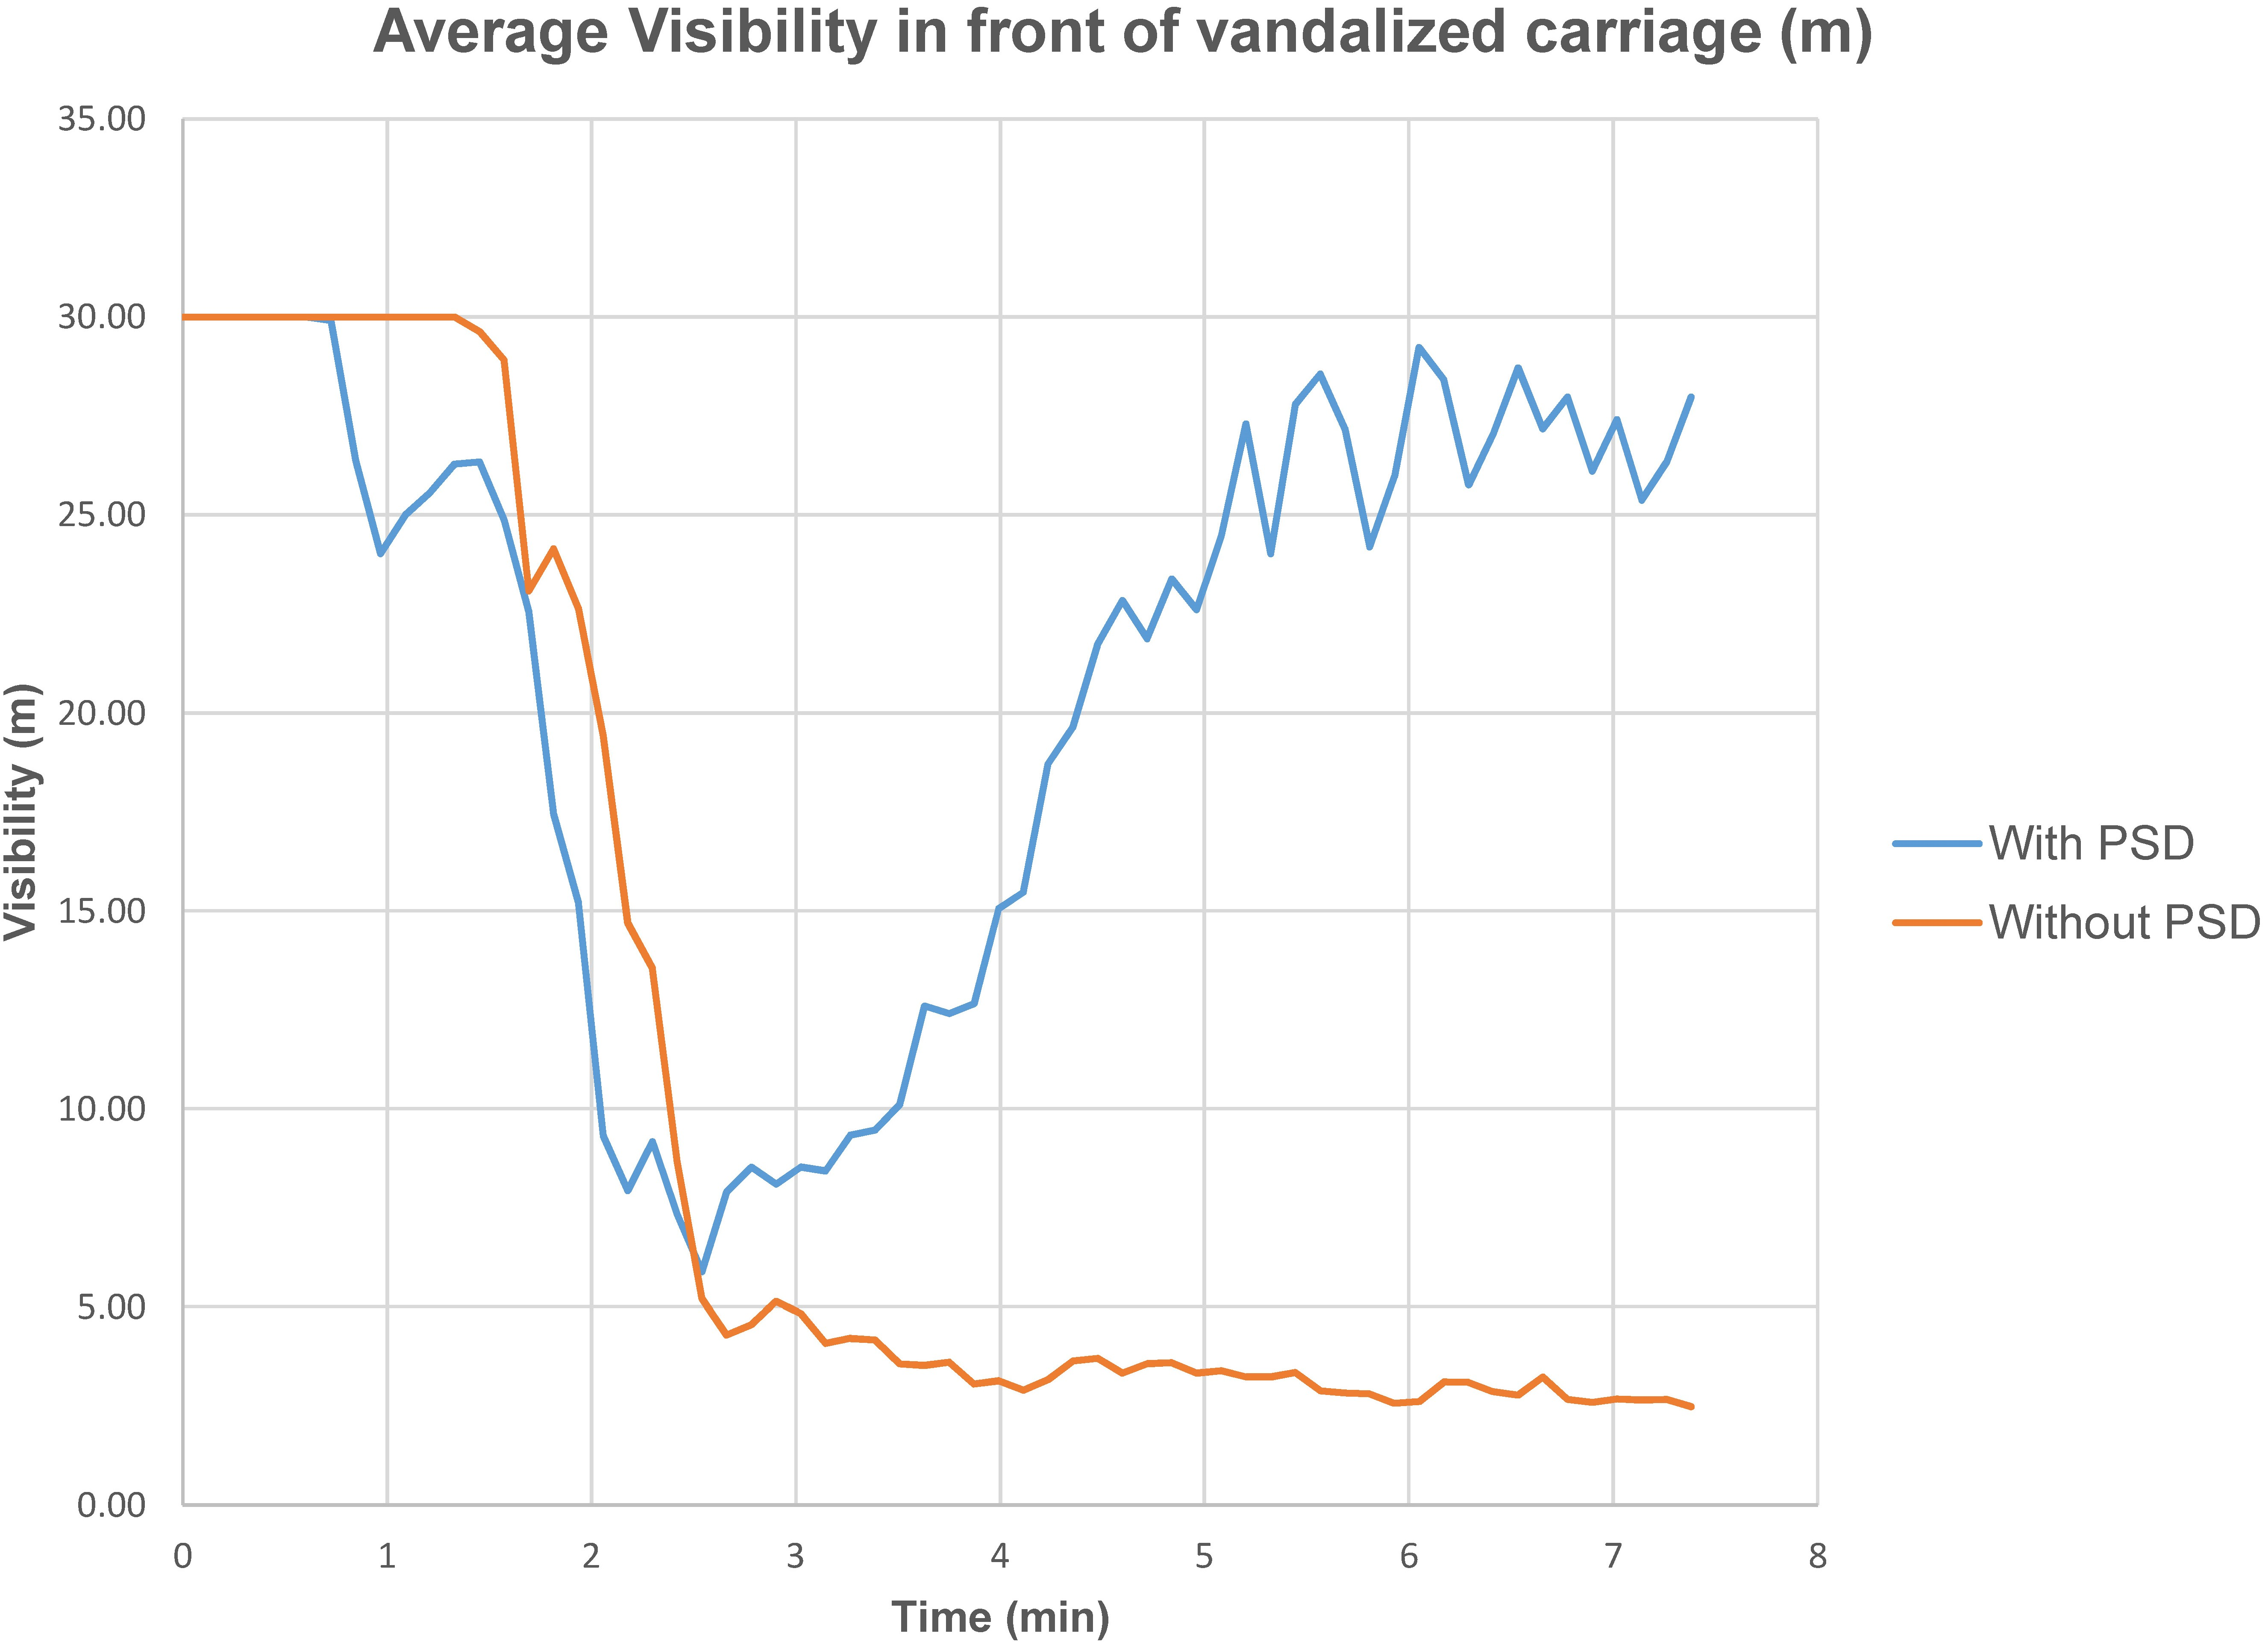
\includegraphics[keepaspectratio=true,width=\dimmin{}{\dimwidth{0.55}}]{images/Fig-4.1.d}{}%mdk
%mdk
\end{mdcenter}%mdk

%mdk-data-line={419}
\begin{mdcenter}%mdk

%mdk-data-line={420}
\noindent\mdline{420}\textbf{Figure 4.1.d. – Average visibility in front of vandalized carriage at a height of 2m.}%mdk
%mdk
\end{mdcenter}%mdk

%mdk-data-line={423}
\noindent\mdline{423}Finally, the comparison of the percentage of platform where visibility is less 
than 10m has great differences between both strategies, as presented in \mdline{424}\textbf{Figure 4.1.e}\mdline{424}.%mdk

%mdk-data-line={426}
\begin{mdcenter}%mdk

%mdk-data-line={427}
\noindent\mdline{427}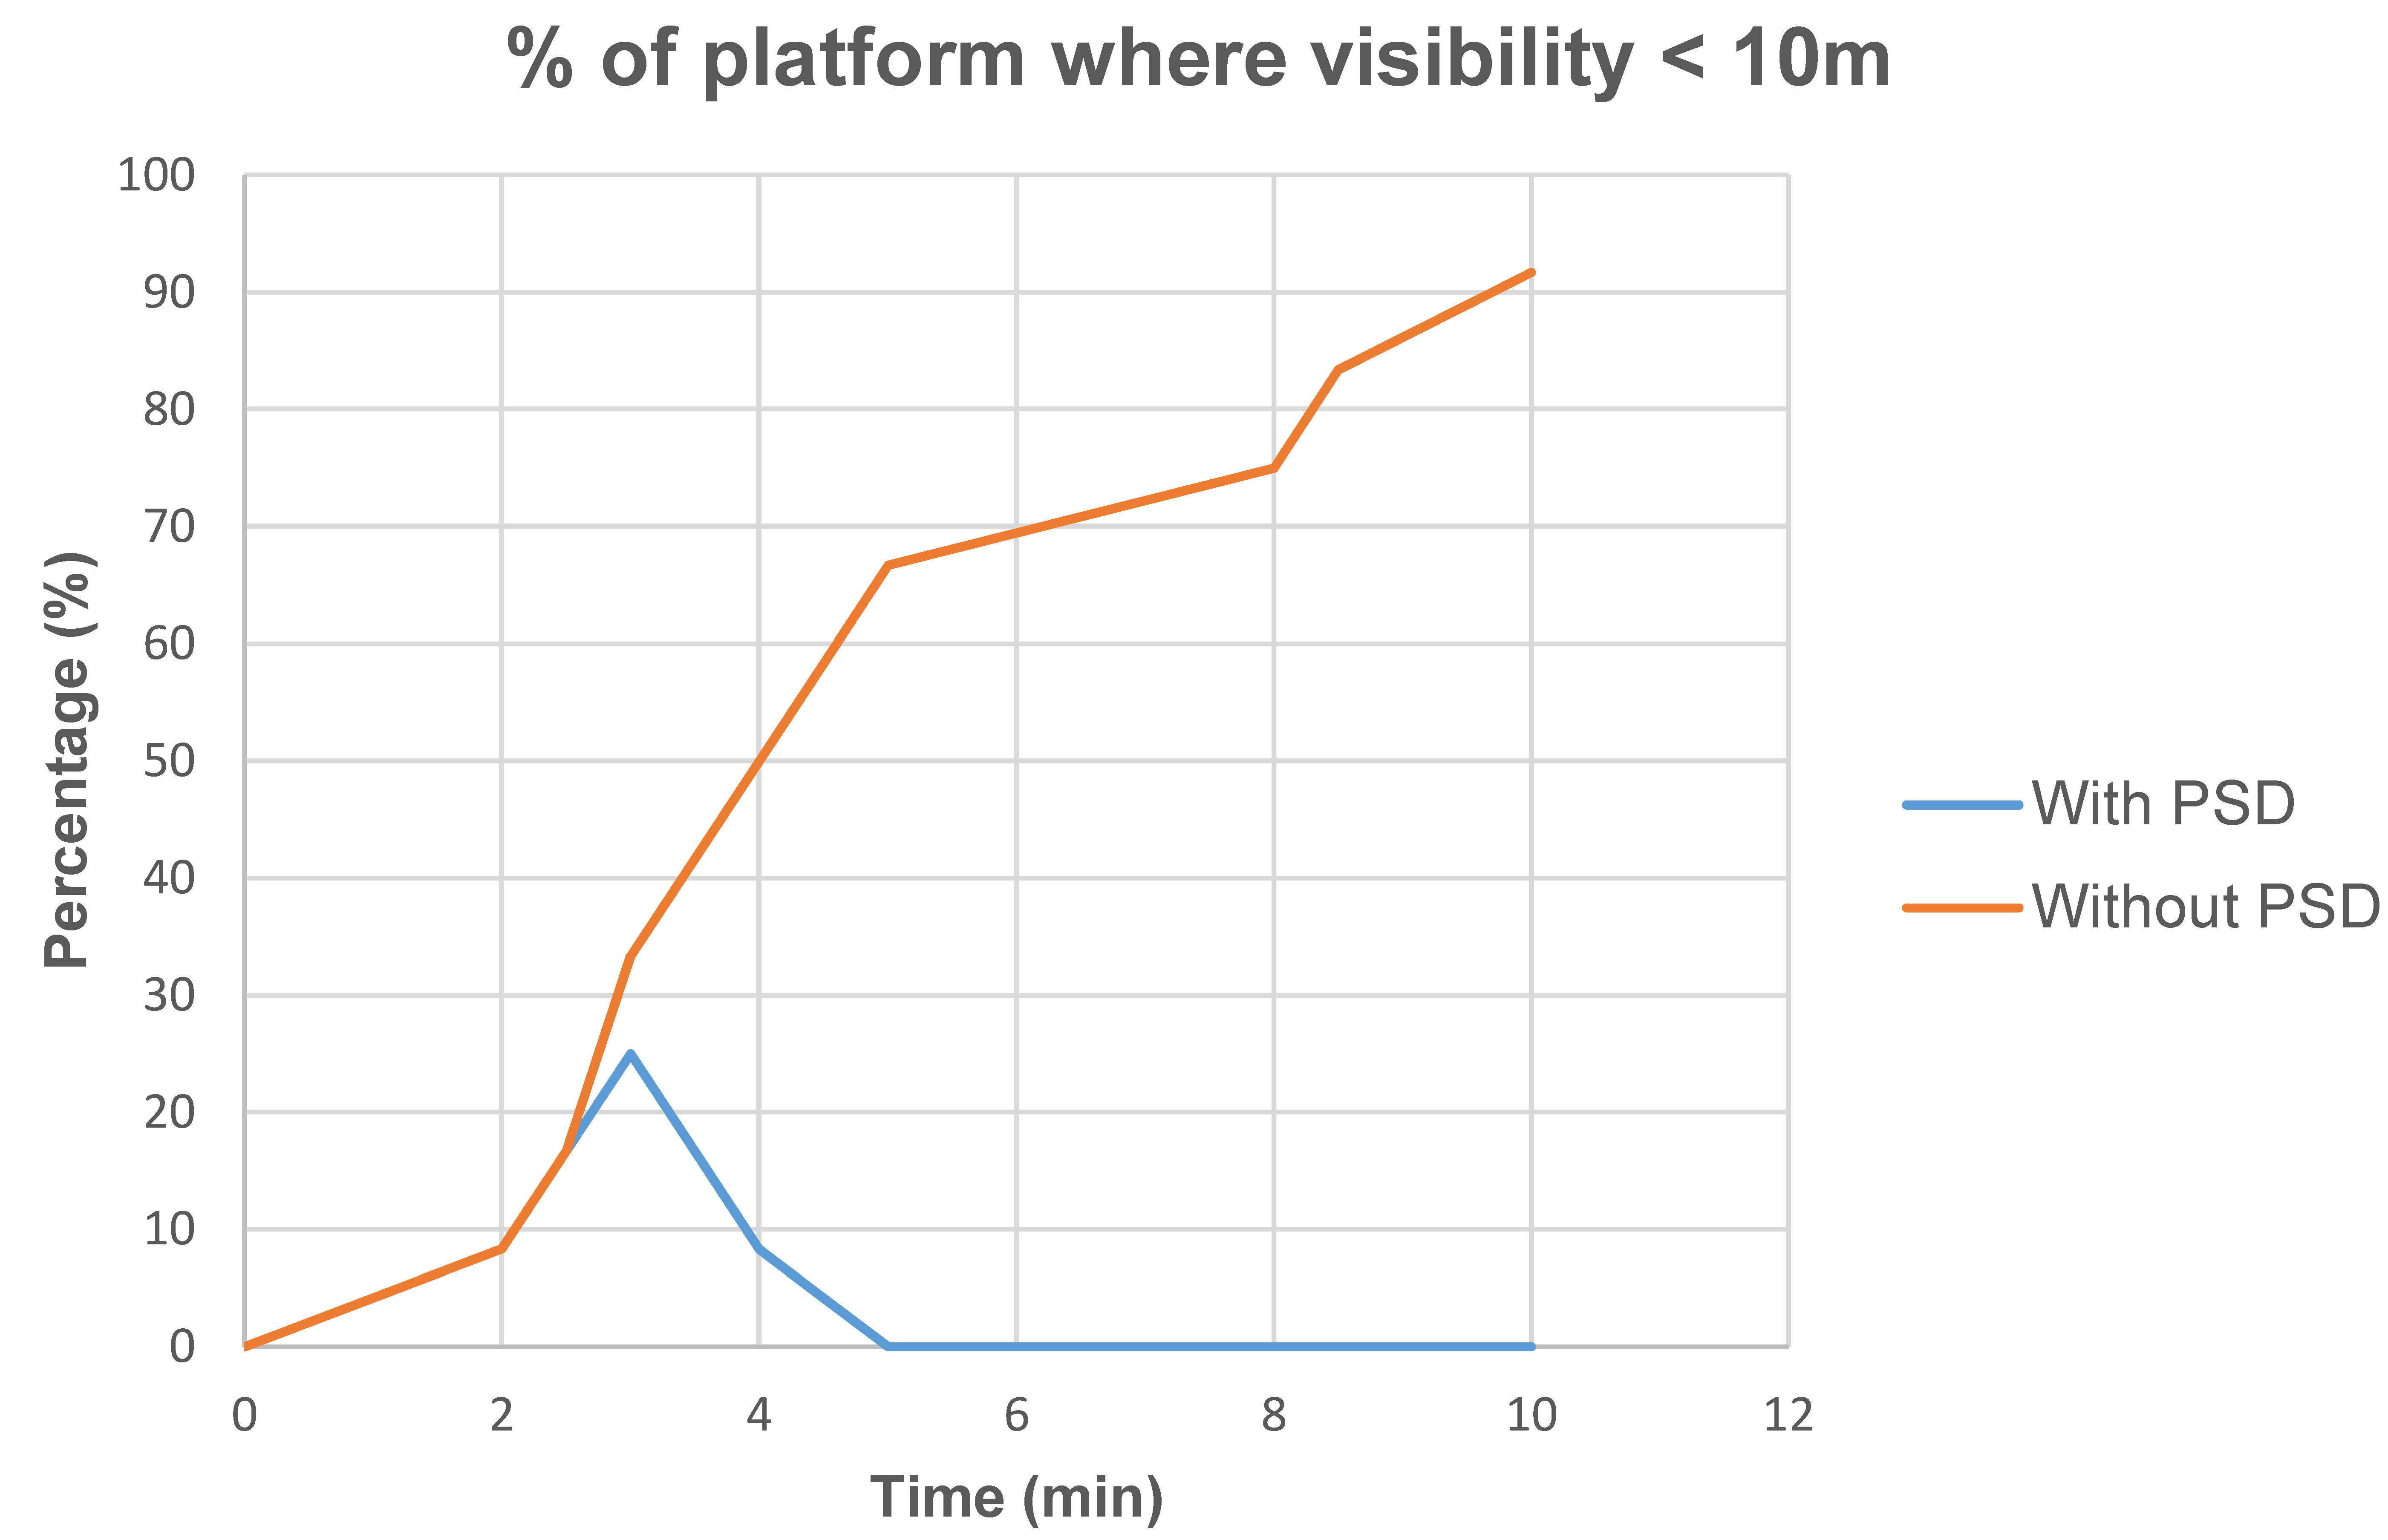
\includegraphics[keepaspectratio=true,width=\dimmin{}{\dimwidth{0.55}}]{images/Fig-4.1.e}{}%mdk
%mdk
\end{mdcenter}%mdk

%mdk-data-line={431}
\begin{mdcenter}%mdk

%mdk-data-line={432}
\noindent\mdline{432}\textbf{Figure 4.1.e. – \% of platform with less than 10m of visibility at a height of 2m.}%mdk
%mdk
\end{mdcenter}%mdk

%mdk-data-line={435}
\begin{itemize}[noitemsep,topsep=\mdcompacttopsep]%mdk

%mdk-data-line={435}
\item\mdline{435}\textbf{Evacuation time}\mdline{435}%mdk
%mdk
\end{itemize}%mdk

%mdk-data-line={437}
\noindent\mdline{437}The evacuation simulation has been done with the software Pathfinder, which 
allows to integrate the FDS results in the evacuation process.%mdk

%mdk-data-line={440}
\mdline{440}The occupation load considered has been 320 passengers in platform PL. A, 320 
passengers in Platform PL.B and 60 passengers in the carriages. Besides, the 
walking speeds have been adapted depending on whether there is smoke in the 
escape route; if it is the case, the values measured by Yin and Yamada have 
been integrated in the model.%mdk

%mdk-data-line={446}
\mdline{446}The pre-movement times for each region of the platforms ranges from 15s to 90s, 
depending on the proximity to the fire. The escalator on the side of the vandalized 
carriage is out of service, as suggested in the NFPA 130.%mdk

%mdk-data-line={450}
\mdline{450}The time needed for the evacuation to the mezzanine level in the case of strategy 
S.T. A was 140 s, while the time required in the case of the strategy S.T. B was 
148 s. Both times are quite similar, because the occupation load is not very high, 
and, due to the absence of queues, the passengers move quickly and are barely 
affected by the smoke with strategy S.T. B.%mdk

%mdk-data-line={456}
\subsection{\mdline{456}4.2.\hspace*{0.5em}\mdline{456}Simulations in Cavern stations}\label{sec-simulations-in-cavern-stations}%mdk%mdk

%mdk-data-line={458}
\noindent\mdline{458}Unlike it has been done in the case of Cut \mdline{458}\&\mdline{458} Cover stations, the study in Cavern 
stations is focused on a geometry where there is only one platform.%mdk

%mdk-data-line={461}
\mdline{461}Some devices for the control of temperature, CO concentration and visibility have 
been placed all along the escape routes. The fire takes place in the last carriage 
on the right, as shown in \mdline{463}\textbf{Figure 4.2.a}\mdline{463}.%mdk

%mdk-data-line={465}
\begin{mdcenter}%mdk

%mdk-data-line={466}
\noindent\mdline{466}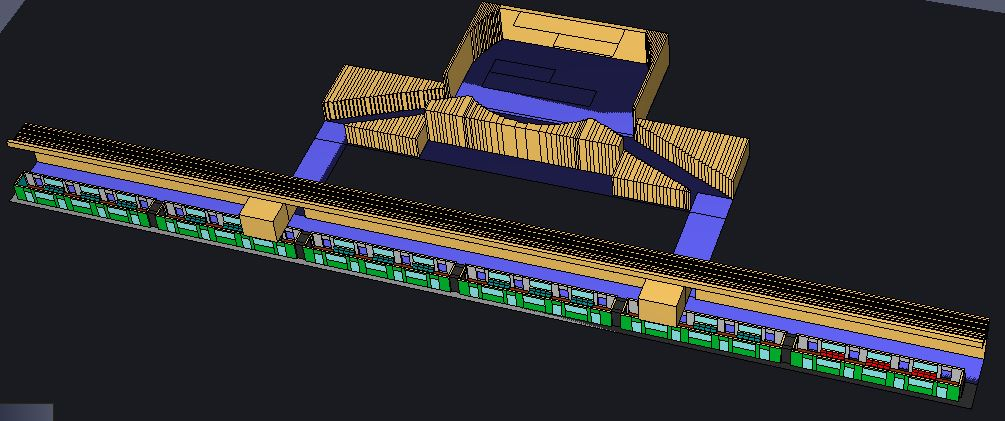
\includegraphics[keepaspectratio=true,width=\dimmin{}{\dimwidth{0.55}}]{images/Fig-4.2.a}{}%mdk
%mdk
\end{mdcenter}%mdk

%mdk-data-line={470}
\begin{mdcenter}%mdk

%mdk-data-line={471}
\noindent\mdline{471}\textbf{Figure 4.2.a. – Cavern fire model created with Pyrosim.}%mdk
%mdk
\end{mdcenter}%mdk

%mdk-data-line={474}
\begin{itemize}[noitemsep,topsep=\mdcompacttopsep]%mdk

%mdk-data-line={474}
\item\mdline{474}\textbf{Main differences between both strategies.}\mdline{474}%mdk
%mdk
\end{itemize}%mdk

%mdk-data-line={476}
\noindent\mdline{476}The volume included in the platform is much smaller than in the case of the 
Cut \mdline{477}\&\mdline{477} Cover station. Then, the main difference between both strategies is the 
fact that, in strategy S.T. A, part of the smoke can be isolated thanks to the 
PSD, while the conditions are much harsher for passengers in strategy S.T. B.%mdk

%mdk-data-line={481}
\begin{itemize}[noitemsep,topsep=\mdcompacttopsep]%mdk

%mdk-data-line={481}
\item\mdline{481}\textbf{Means of egress.}\mdline{481}%mdk
%mdk
\end{itemize}%mdk

%mdk-data-line={483}
\noindent\mdline{483}The passengers have four means of egress:%mdk

%mdk-data-line={485}
\begin{itemize}[noitemsep,topsep=\mdcompacttopsep]%mdk

%mdk-data-line={485}
\item\mdline{485}Emergency door on the right side of the platform.%mdk

%mdk-data-line={486}
\item\mdline{486}Passageway on the right side of the platform.%mdk

%mdk-data-line={487}
\item\mdline{487}Passageway on the left side of the platform.%mdk

%mdk-data-line={488}
\item\mdline{488}Emergency door on the left side of the platform.%mdk
%mdk
\end{itemize}%mdk

%mdk-data-line={490}
\noindent\mdline{490}The region in front of the vandalized carriage is the one most affected by the fire.%mdk

%mdk-data-line={492}
\begin{itemize}[noitemsep,topsep=\mdcompacttopsep]%mdk

%mdk-data-line={492}
\item\mdline{492}\textbf{Development of the fire.}\mdline{492}%mdk
%mdk
\end{itemize}%mdk

%mdk-data-line={494}
\noindent\mdline{494}The beginning of the fire is similar to the case of Cut \mdline{494}\&\mdline{494} Cover stations: the smoke 
manages to get to every carriage, since they are connected to each other. Besides, 
the windows on both sides of the vandalized carriage break out when the temperature 
of 470ºC is reached.%mdk

%mdk-data-line={499}
\mdline{499}Since the volume of the platform is smaller with respect to the previous case, 
the levels of temperature inside and in front of the vandalized carriage surpass 
the lethal levels, as shown in \mdline{501}\textbf{Figure 4.2.a}\mdline{501}, but no passenger is likely to remain 
the required time to become incapacitated.%mdk

%mdk-data-line={505}
\begin{mdcenter}%mdk

%mdk-data-line={506}
\noindent\mdline{506}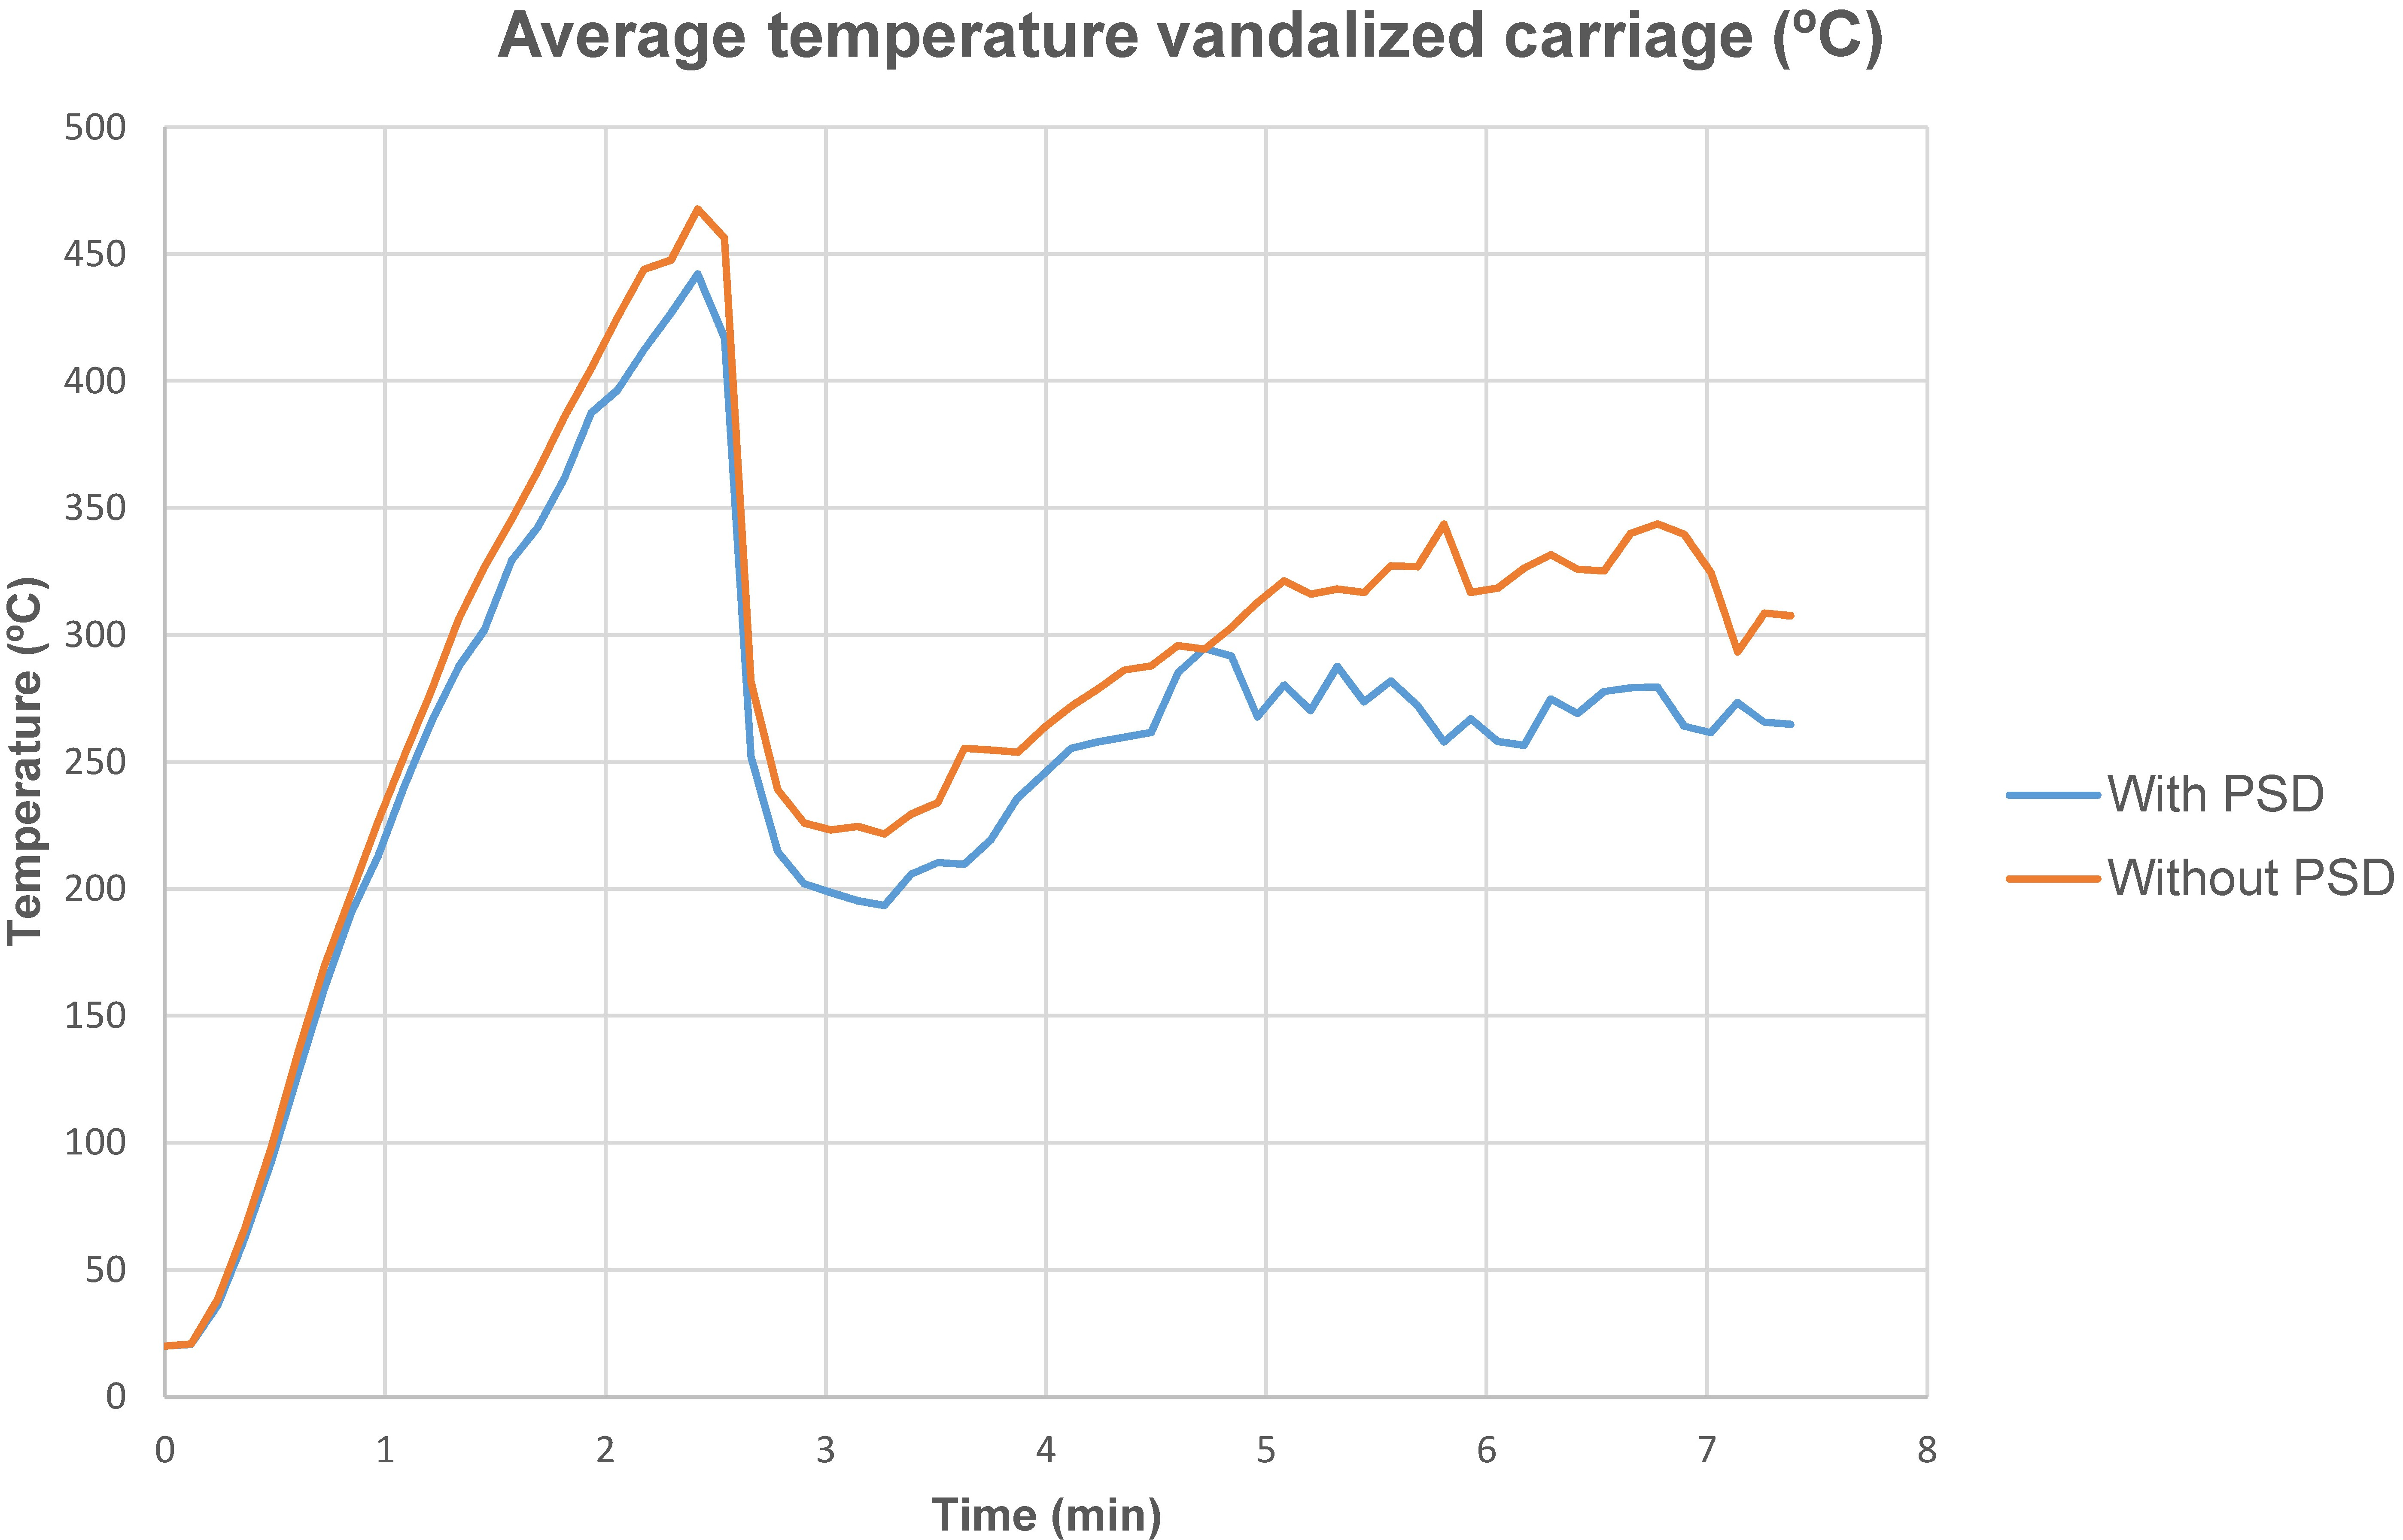
\includegraphics[keepaspectratio=true,width=\dimmin{}{\dimwidth{0.55}}]{images/Fig-4.2.b}{}%mdk
%mdk
\end{mdcenter}%mdk

%mdk-data-line={510}
\begin{mdcenter}%mdk

%mdk-data-line={511}
\noindent\mdline{511}\textbf{Figure 4.2.b. – Average temperature in the vandalized carriage.}%mdk
%mdk
\end{mdcenter}%mdk

%mdk-data-line={514}
\noindent\mdline{514}The maximum temperature registered in the platform without PSD is 200ºC, but 
at a height far from any passenger, as presented in \mdline{515}\textbf{Figure 4.2.c}\mdline{515}. In contrast, 
the maximum temperature on the platform, with PSD at a height of 2m is 80ºC, 
but close to the vandalized carriage.%mdk

%mdk-data-line={520}
\begin{mdcenter}%mdk

%mdk-data-line={521}
\noindent\mdline{521}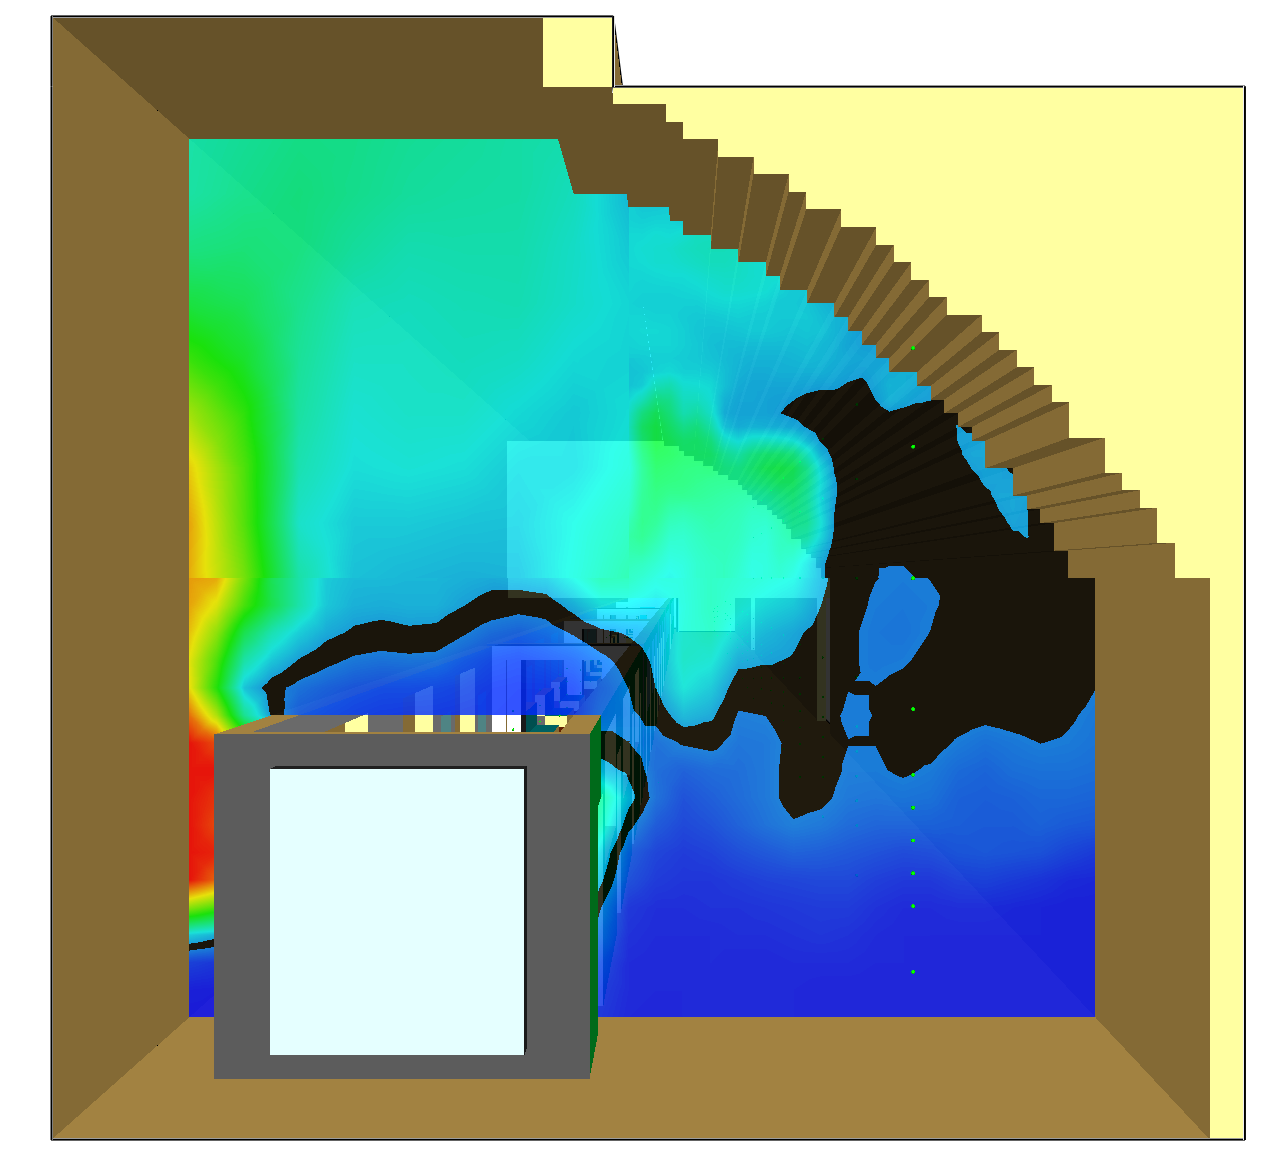
\includegraphics[keepaspectratio=true,width=\dimmin{}{\dimwidth{0.45}}]{images/Fig-4.2.c}{}%mdk
%mdk
\end{mdcenter}%mdk

%mdk-data-line={525}
\begin{mdcenter}%mdk

%mdk-data-line={526}
\noindent\mdline{526}\textbf{Figure 4.2.c. – Temperature in Cavern stations without PSD (t=6min, 80ºC in bold).}%mdk
%mdk
\end{mdcenter}%mdk

%mdk-data-line={530}
\noindent\mdline{530}However, the visibility is quite affected because of the spread of the smoke, as 
it is shown in \mdline{531}\textbf{Figure 4.2.d}\mdline{531} in the region of the platform in front of the vandalized 
carriage, as it is where the conditions are harder.%mdk

%mdk-data-line={534}
\begin{mdcenter}%mdk

%mdk-data-line={535}
\noindent\mdline{535}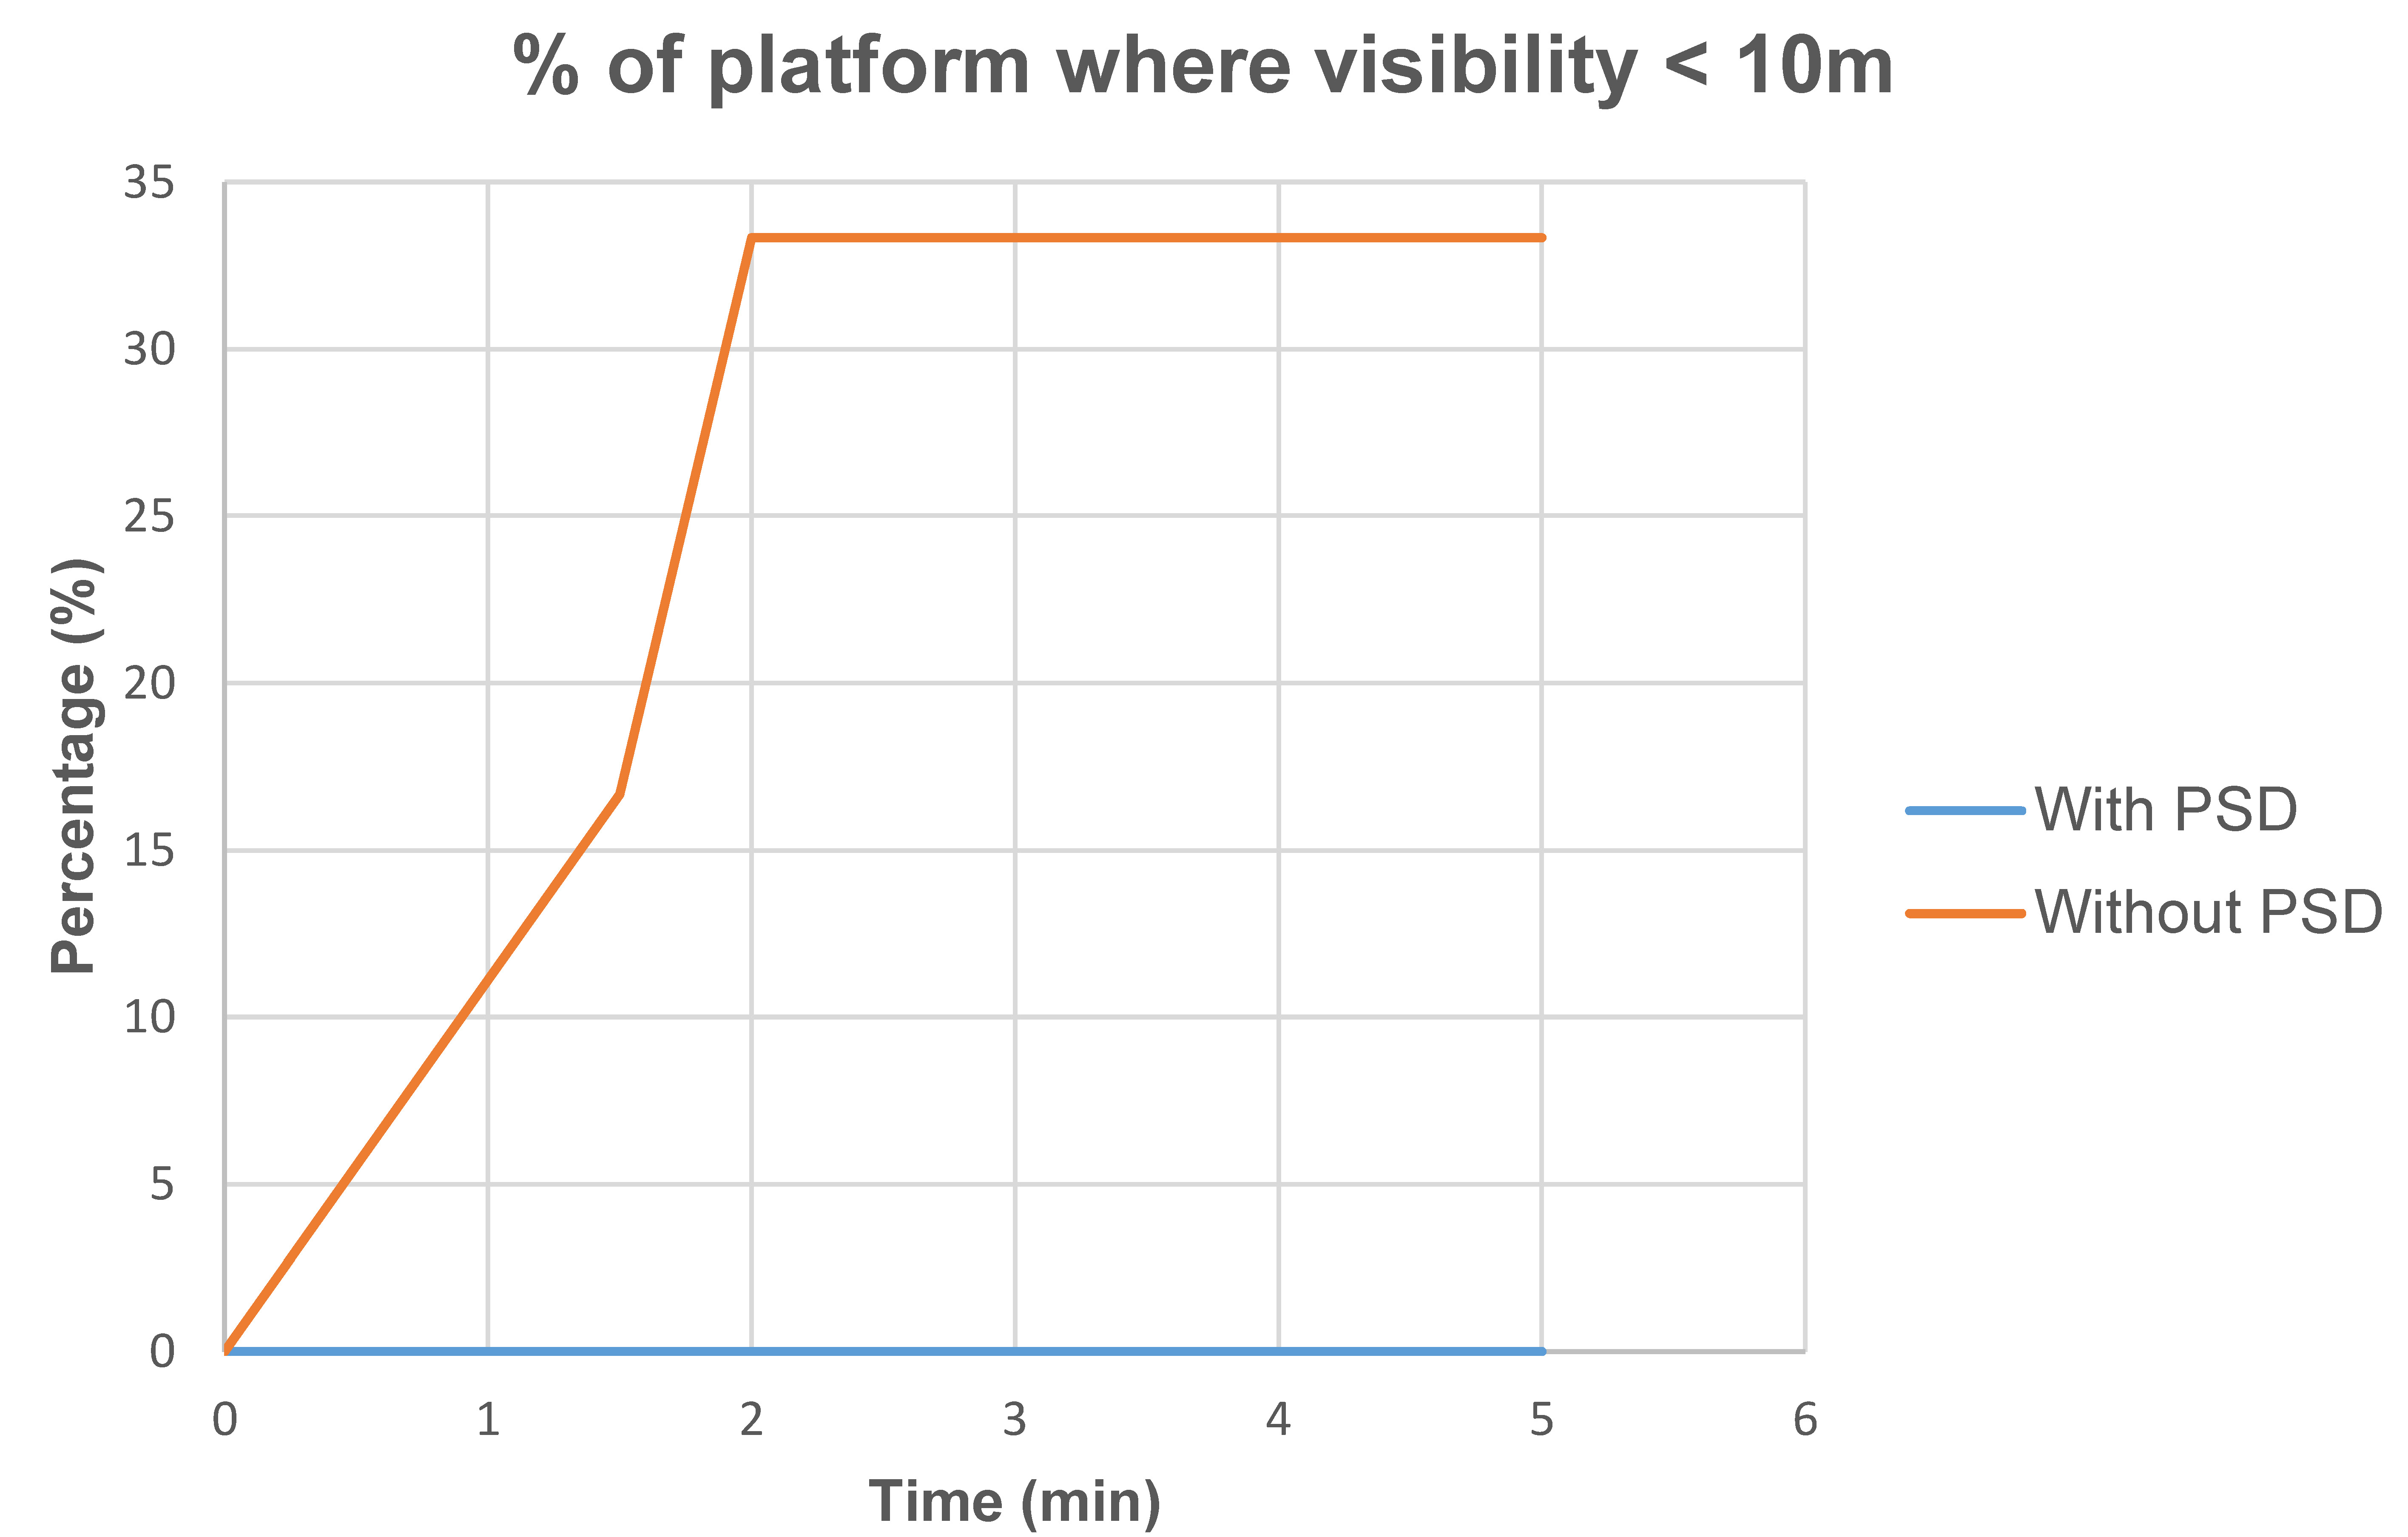
\includegraphics[keepaspectratio=true,width=\dimmin{}{\dimwidth{0.55}}]{images/Fig-4.2.d}{}%mdk
%mdk
\end{mdcenter}%mdk

%mdk-data-line={539}
\begin{mdcenter}%mdk

%mdk-data-line={540}
\noindent\mdline{540}\textbf{Figure 4.2.d. – Average visibility in front of vandalized carriage.}%mdk
%mdk
\end{mdcenter}%mdk

%mdk-data-line={543}
\noindent\mdline{543}The comparison between \% of platform with less than 10m of visibility offers 
great differences, as presented in \mdline{544}\textbf{Figure 4.2.e}\mdline{544}.%mdk

%mdk-data-line={546}
\begin{mdcenter}%mdk

%mdk-data-line={547}
\noindent\mdline{547}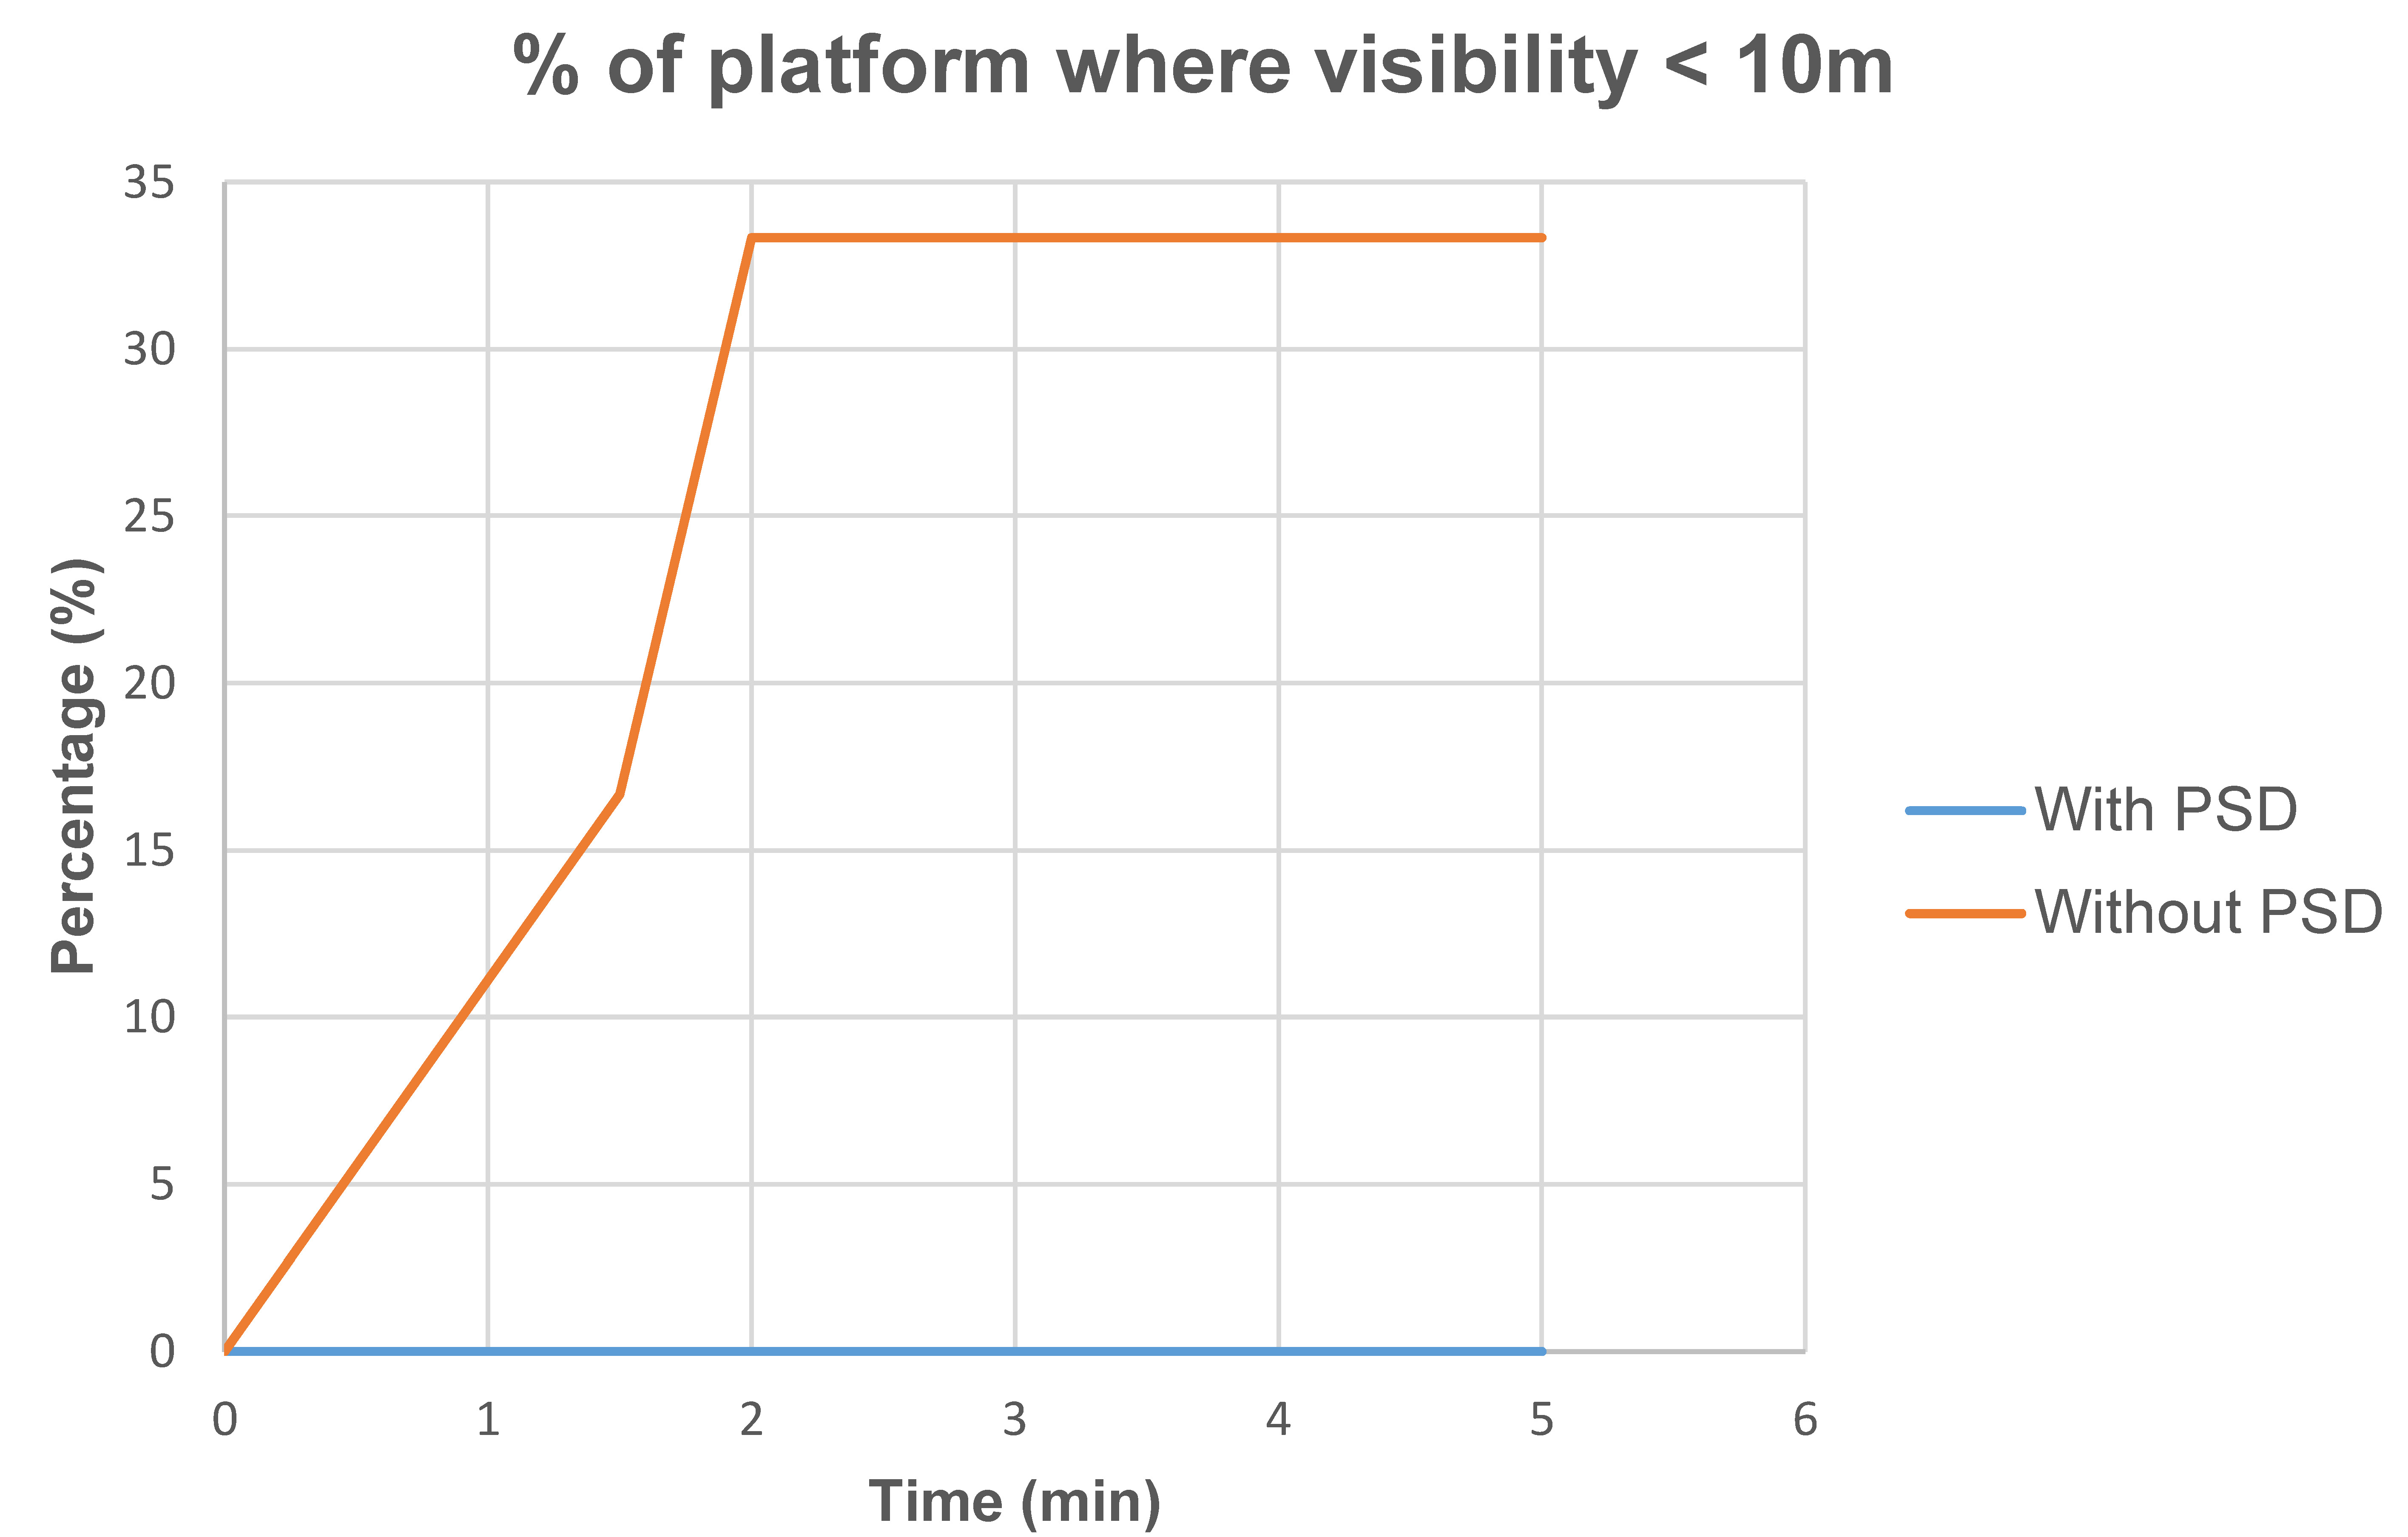
\includegraphics[keepaspectratio=true,width=\dimmin{}{\dimwidth{0.55}}]{images/Fig-4.2.e}{}%mdk
%mdk
\end{mdcenter}%mdk

%mdk-data-line={551}
\begin{mdcenter}%mdk

%mdk-data-line={552}
\noindent\mdline{552}\textbf{Figure 4.2.e. – \% of platform with less than 10m of visibility at a height of 2m.}%mdk
%mdk
\end{mdcenter}%mdk

%mdk-data-line={555}
\begin{itemize}[noitemsep,topsep=\mdcompacttopsep]%mdk

%mdk-data-line={555}
\item\mdline{555}\textbf{Evacuation time.}\mdline{555}%mdk
%mdk
\end{itemize}%mdk

%mdk-data-line={557}
\noindent\mdline{557}The software Pathfinder has been used as well for this simulation. The occupation 
load considered is 320 passengers in the platform and 60 passengers in the train.%mdk

%mdk-data-line={560}
\mdline{560}In this case, the walking speeds have also been adapted to situations with 
presence of smoke in the escape routes, taking into account the values from 
Yin and Yamada. Besides, the comparison has been done on the time needed to 
reach either an emergency door or one of the passageways, unlike in the previous 
case where the goal was to reach the mezzanine level.%mdk

%mdk-data-line={566}
\mdline{566}The pre-movement times range from 15s to 100s, depending on the location of the 
passengers, since the ones who are far will have more trouble to see the smoke.%mdk

%mdk-data-line={569}
\mdline{569}The time required for the complete evacuation in the case where the strategy 
S.T. A was applied was 121 s, while in the case where strategy S.T. B was adopted, 
the time needed was 116 s.%mdk

%mdk-data-line={573}
\mdline{573}As in the case of the Cut \mdline{573}\&\mdline{573} Cover station, the difference is quite reduced, and the 
reason for these values is that the occupation load is not very high. Thus, the 
passengers manage to get to a safe place quickly, without being interrupted in their 
route. Moreover, the pre-movement time is defined by a statistical distribution, what 
means that the result will be slightly different every time one makes a simulation.%mdk

%mdk-data-line={579}
\mdline{579}Furthermore, in this particular case, no passenger has used the emergency door close 
to the vandalized carriage, since the conditions are very hard there. This means that 
nobody remains in a queue, but the majority of passengers evacuate through the 
passageways, with a 5m – width, offering a great capacity for the evacuation purposes.%mdk

%mdk-data-line={584}
\section{\mdline{584}5.\hspace*{0.5em}\mdline{584}Conclusions}\label{sec-conclusions}%mdk%mdk

%mdk-data-line={586}
\noindent\mdline{586}After this study, it is possible to extract some conclusions from it.%mdk

%mdk-data-line={588}
\mdline{588}First, it has been demonstrated that the occupation load is a key factor on 
evacuation, since, the more people to evacuate, the more likely people will have 
to deal with smoke while trying to get to a safe place.%mdk

%mdk-data-line={592}
\mdline{592}Second, although PSD are installed to have an automatic operation of the trains in a 
subway station, it has been demonstrated that they provide better evacuation 
conditions in an emergency situation, since they isolate part of the smoke.%mdk

%mdk-data-line={596}
\mdline{596}Third, an advantage of PSD is that they make compatible an operation with station 
and tunnel ventilation simultaneously. This allows to optimize this operation and 
provides air velocity opposite to the egress direction of the passengers, which is 
positive in terms of safety.%mdk

%mdk-data-line={601}
\mdline{601}Finally, the time for the detection of a fire is another aspect of great relevancy, 
as it makes the exhaust system to get activated. The higher the delay of detection 
is, the more dangerous the situation turns out to be.%mdk

%mdk-data-line={605}
\section{\mdline{605}6.\hspace*{0.5em}\mdline{605}Bibliography and references}\label{sec-bibliography-and-references}%mdk%mdk

%mdk-data-line={607}
\noindent\mdline{607}[1]\mdline{607} National Fire Protection Association (NFPA) 130, Standard for Fixed Guideway Transit 
and Passenger Rail Systems, 2014 Edition.%mdk

%mdk-data-line={610}
\mdline{610}[2]\mdline{610} National Fire Protection Association (NFPA) 92, Standard for Smoke Control Systems, 
2012 Edition.%mdk

%mdk-data-line={613}
\mdline{613}[3]\mdline{613} British Standard BS 7974:2001, Application of fire safety engineering principles 
to the design of buildings – Code of practice.%mdk

%mdk-data-line={616}
\mdline{616}[4]\mdline{616} Model Scale Railcar Fire Tests. Brandforskproject 404-011 (Haukur Ingason).%mdk

%mdk-data-line={618}
\mdline{618}[5]\mdline{618} Full-scale fire tests with a commuter train in a tunnel (Anders Lönnermark, 
Alexander Claesson, Johan Lindström, Ying Zhen Li, Mia Kumm, Haukur Ingason).%mdk

%mdk-data-line={621}
\mdline{621}[6]\mdline{621} Estudio de preinversión a nivel de perfil de la línea 4 de metro de Lima. 
Ventilation design report.%mdk%mdk


\end{document}
